\documentclass[aps,prb,twocolumn,superscriptaddress,longbibliography]{revtex4-2}

\usepackage{graphicx}
\usepackage{amsmath}
\usepackage{amssymb}
\usepackage{bm}
\usepackage{color}

\begin{document}

\title{Quantum Teleportation and Super Dense Coding in Open Quantum Systems}

\author{R Afzali}
\author{A. H Asghari}


\date{\today}

\begin{abstract}
Quantum communication protocols rely critically on the preservation of entanglement and quantum coherence in realistic noisy environments. In this work, we investigate quantum teleportation and dense coding using correlated electron pairs described within a Hubbard--Bogoliubov--de Gennes framework and subjected to non-Markovian open-system dynamics. The superconducting correlations are obtained self-consistently, and the corresponding normal and anomalous Green's functions are employed to construct spatially dependent two-qubit density matrices. The resulting states are evolved using Kraus-operator descriptions of environmental noise, including non-Markovian amplitude damping and dephasing channels. The robustness of the quantum resources is characterized through concurrence and singlet-referenced Uhlmann fidelity, while the Holevo quantity of an equal-probability Pauli encoding ensemble is used to quantify the information available to the corresponding dense-coding protocol. For two representative non-Markovian amplitude-damping regimes, the results reveal a pronounced dependence of quantum correlations on both the spatial separation of the electron pair and the evolution time. Environmental coupling suppresses the initially available entanglement and communication resources, while the nonmonotonic survival probability produces transient revivals of concurrence and singlet fraction. The Pauli-ensemble Holevo quantity evolves differently and approaches the one-bit limit of the long-time amplitude-damped product state. A converged interaction sweep at $U/t=40$, $75$, and $115$ shows that the Hubbard interaction changes the initial spatial profiles and hence the subsequent fidelity and Holevo dynamics, but their ordering with $U$ is separation dependent rather than uniformly enhancing or suppressing. A separate density-resolved initial-state study at $U/t=15$ and $25$ finds nonzero-gap stationary branches at every sampled filling for $U/t=15$, and for $n\geq1$ on the production mesh for $U/t=25$. Nevertheless, none of the 140 tested nonzero lattice-site resources has nonzero concurrence or average teleportation fidelity above $2/3$. The legacy dynamics use the repository's magnitude-amplitude Green's-function reduction; the new density study uses the corrected signed equal-time construction and is not used to reinterpret those archived time-dependent results.
\end{abstract}

\pacs{74.20.Fg, 03.67.Mn, 03.65.Ud, 74.25.-q}

\maketitle

\section{Introduction}

Entanglement converts a shared bipartite state into an operational resource for quantum communication. In quantum teleportation, a maximally entangled pair together with two classical bits enables the transfer of an unknown qubit state without physically transmitting the carrier of that state~\cite{Bennett1993}. In superdense coding, the same elementary resource allows one qubit to convey up to two bits of classical information~\cite{BennettWiesner1992}. In realistic settings, however, quantum resources are generally mixed and interact with their surrounding environments. Their usefulness must therefore be characterized through state-dependent quantities such as concurrence, fidelity, and encoded Holevo information~\cite{Wootters1998,Jozsa1994,Bruss2004}.

Superconductors provide a natural many-body setting in which fermionic pairing generates strong quantum correlations between electrons. Within Bardeen--Cooper--Schrieffer and Bogoliubov--de Gennes descriptions, normal and anomalous Green functions encode the spatial structure of these paired states~\cite{Oh2004,Oh2005}. Reduced two-particle spin states can consequently be reconstructed from the corresponding correlation functions and treated as potential resources for quantum communication. This microscopic approach differs from assuming an idealized Bell pair from the outset, since the resulting entanglement is determined by the underlying electronic dispersion, superconducting pairing symmetry, interaction strength, and electron filling. The spatial dependence of the Green functions further makes it possible to investigate how the available quantum correlations vary with the separation between the two electrons.

Environmental memory introduces an additional layer of complexity. For a qubit coupled to a structured reservoir with a Lorentzian spectral density, the excited-state survival probability can exhibit oscillatory behavior, leading to memory-induced revivals of quantum correlations that would otherwise decay monotonically in a Markovian description~\cite{Breuer2002,Bellomo2007}. Combining a spatially structured superconducting source with non-Markovian quantum channels therefore provides a framework for investigating how microscopic pairing correlations survive, decay, and re-emerge in the presence of environmental noise. In particular, it allows one to study how the usefulness of the superconducting two-particle state for quantum communication depends simultaneously on spatial separation and evolution time.

Here, we develop and numerically investigate such a framework. We first solve an extended-Hubbard Bogoliubov--de Gennes model on a square lattice and evaluate the associated equal-time normal and anomalous Green functions. These correlation functions are then used to reconstruct normalized two-spin X states for electron pairs separated by different distances and directions in real space. The resulting two-qubit states are subsequently evolved under open-system quantum channels describing independent or correlated environmental interactions, with particular attention to non-Markovian amplitude damping.

The evolution of the superconducting quantum resource is characterized using several complementary quantities. Concurrence is employed to quantify bipartite entanglement, while purity and von Neumann entropy describe the degree of mixedness generated by environmental interactions. Uhlmann fidelity to the initial state monitors the preservation of that state during the open-system evolution. Separately, the overlap with the spin singlet quantifies the retention of singlet weight; for a pure singlet reference it coincides with the pure-state-referenced Uhlmann fidelity, but it is not automatically an optimized teleportation fidelity. For dense coding, we evaluate the Holevo quantity associated with the standard equal-probability Pauli encoding operations and derive its reduction to an entropy expression involving the two-qubit state and one reduced subsystem.

This framework therefore connects microscopic superconducting correlations with quantities relevant to quantum communication. By examining their joint spatial, angular, temporal, and interaction dependence, we investigate how the structure of the superconducting state and non-Markovian environmental effects influence the persistence and possible revival of entanglement, singlet weight, and dense-coding performance.


\section{Model and Methods}

\subsection{Lattice Hamiltonian and self-consistent BdG solution}


The superconducting system is described on a two-dimensional square lattice
with two helicity- or spin-resolved branches, denoted by $s=\pm1$.
The normal-state dispersion is written as

\begin{equation}
\epsilon_{\mathbf{k}s}
=
-2t(\cos k_x+\cos k_y)
-2sV_{\mathrm{SO}}
\sqrt{\sin^2 k_x+\sin^2 k_y},
\label{eq:dispersion}
\end{equation}

where $t$ denotes the nearest-neighbor hopping amplitude and
$V_{\mathrm{SO}}$ represents the spin-orbit coupling strength.

The superconducting gap contains both on-site and extended-$s$-wave
contributions and is expressed as

\begin{equation}
\Delta_{\mathbf{k}s}
=
\Delta_0
-
\frac{\Delta_s}{4t}\epsilon_{\mathbf{k}s},
\label{eq:gap}
\end{equation}

where $\Delta_0$ and $\Delta_s$ denote the corresponding superconducting
order parameters. The momentum dependence of the gap therefore follows
directly from the electronic dispersion.

The quasiparticle excitation energy is

\begin{equation}
E_{\mathbf{k}s}
=
\sqrt{
\left(\epsilon_{\mathbf{k}s}-\mu\right)^2
+
\Delta_{\mathbf{k}s}^{\,2}
},
\label{eq:quasiparticle_energy}
\end{equation}

where $\mu$ is the chemical potential. The corresponding coherence factors
are given by

\begin{equation}
u_{\mathbf{k}s}^{2}
=
\frac{1}{2}
\left(
1+
\frac{\epsilon_{\mathbf{k}s}-\mu}
{E_{\mathbf{k}s}}
\right),
\qquad
v_{\mathbf{k}s}^{2}
=
\frac{1}{2}
\left(
1-
\frac{\epsilon_{\mathbf{k}s}-\mu}
{E_{\mathbf{k}s}}
\right).
\label{eq:coherence_factors}
\end{equation}

The superconducting order parameters and chemical potential are determined
self-consistently. The equations solved numerically are

\begin{equation}
0
=
\Delta_0
+
\frac{1}{8N_k^2}
\sum_{\mathbf{k},s}
V_{\mathbf{k}s}
\frac{\Delta_{\mathbf{k}s}}
{E_{\mathbf{k}s}}
\tanh
\left(
\frac{\beta E_{\mathbf{k}s}}{2}
\right),
\label{eq:self_consistent_delta0}
\end{equation}

\begin{equation}
0
=
\Delta_s
+
\frac{V_1}{N_k^2}
\sum_{\mathbf{k},s}
\frac{\Delta_{\mathbf{k}s}}
{E_{\mathbf{k}s}}
\tanh
\left(
\frac{\beta E_{\mathbf{k}s}}{2}
\right),
\label{eq:self_consistent_deltas}
\end{equation}

and

\begin{equation}
0
=
\frac{1}{2N_k^2}
\sum_{\mathbf{k},s}
\frac{\epsilon_{\mathbf{k}s}-\mu}
{E_{\mathbf{k}s}}
\tanh
\left(
\frac{\beta E_{\mathbf{k}s}}{2}
\right)
-
(1-n),
\label{eq:number_equation}
\end{equation}

where $n$ denotes the electronic filling and
$\beta=1/(k_{\mathrm B}T)$. The momentum-dependent interaction entering
Eq.~\eqref{eq:self_consistent_delta0} is

\begin{equation}
V_{\mathbf{k}s}
=
U
+
8V_1 s_{\mathbf{k}}
+
4\frac{V_1}{t}
V_{\mathrm{SO}}s\lambda_{\mathbf{k}},
\label{eq:interaction}
\end{equation}

with

\begin{equation}
\lambda_{\mathbf{k}}
=
\sqrt{\sin^2 k_x+\sin^2 k_y},
\qquad
s_{\mathbf{k}}
=
\frac{\cos k_x+\cos k_y}{2}.
\label{eq:lambda_sk}
\end{equation}

Here, $U$ denotes the on-site Hubbard interaction strength and $V_1$ characterizes
the extended pairing contribution. In the numerical implementation,
$V_1$ corresponds to the parameter denoted by \texttt{Delta\_t}.
Equations~\eqref{eq:self_consistent_delta0}--\eqref{eq:number_equation}
are solved simultaneously using a multidimensional root-finding procedure.
The calculations employ a $100\times100$ momentum-space grid and are
performed at $T=0$. Unless stated otherwise, the fixed model parameters are
$\Delta_t/t=4.5$, $V_{\mathrm{SO}}=0$, and $n=1.875$; thus the two helicity
branches coincide in the archived calculations. Energies are expressed in
units of $t$, separations in units of the lattice constant, and times in units
of $\hbar/t$.

To examine how the interaction strength modifies the superconducting state,
we evaluate the momentum-dependent gap $\Delta_{\mathbf{k}s}$ throughout
the Brillouin zone for three representative interaction strengths,
$U/t=40$, $75$, and $115$. For each interaction strength,
$\Delta_0$, $\Delta_s$, and $\mu$ are obtained independently from the
self-consistent equations before evaluating Eq.~\eqref{eq:gap}.

\begin{figure*}[t]
    \centering
    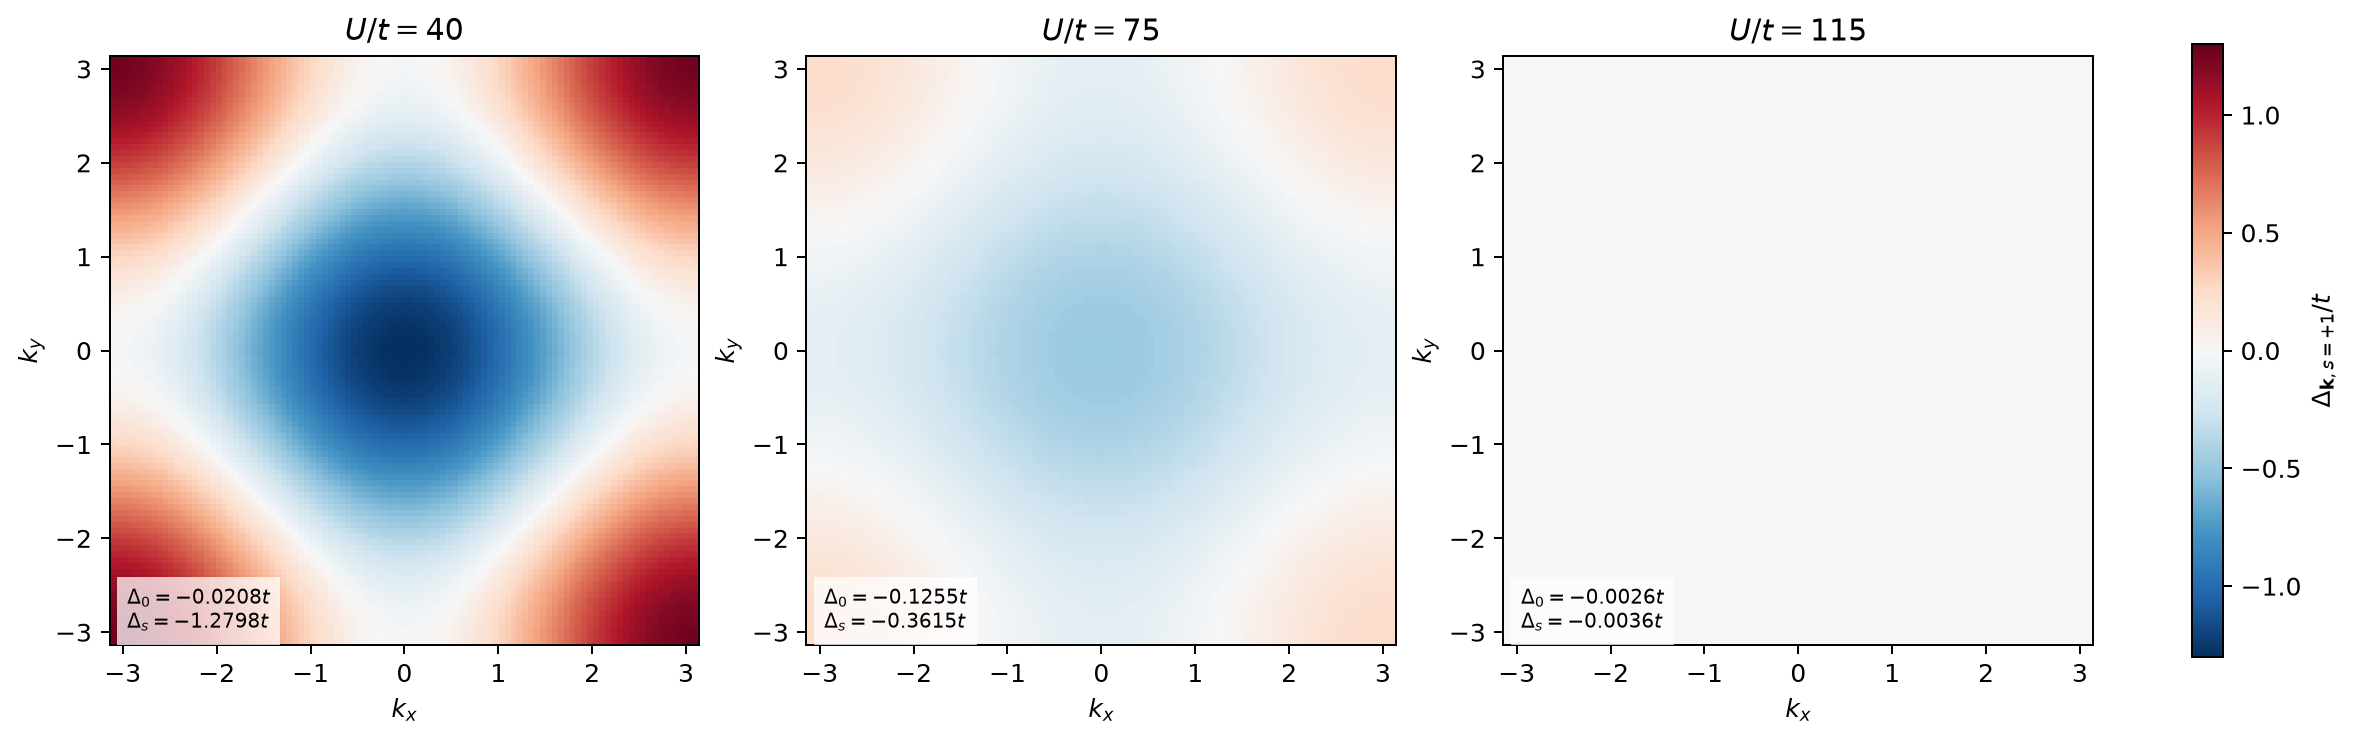
\includegraphics[width=\textwidth]{Delta_ks_heatmaps.png}
    \caption{
    Momentum-space distribution of the implemented superconducting pairing gap
    $\Delta_{\mathbf{k},s=+1}$ over the Brillouin zone for
    $U/t=40$, $75$, and $115$, with a common color scale.
    For each interaction strength, the superconducting order parameters
    $\Delta_0$ and $\Delta_s$, together with the chemical potential $\mu$,
    are obtained independently from
    Eqs.~\eqref{eq:self_consistent_delta0}--\eqref{eq:number_equation}.
    The fixed parameters are $\Delta_t/t=4.5$, $V_{\mathrm{SO}}=0$,
    $n=1.875$, $N_k=100$, and $T=0$. The momentum dependence originates
    from the extended-$s$-wave contribution in Eq.~\eqref{eq:gap}.
    }
    \label{fig:delta_ks_heatmaps}
\end{figure*}

Figure~\ref{fig:delta_ks_heatmaps} shows that
$\Delta_{\mathbf{k}s}$ exhibits a pronounced momentum dependence across
the Brillouin zone. This structure follows from the dependence of the gap
on $\epsilon_{\mathbf{k}s}$ through Eq.~\eqref{eq:gap}. The resulting
pattern reflects the extended-$s$-wave contribution and preserves the
symmetry of the underlying square-lattice dispersion.

For $U/t=40$, the reproduced self-consistent solution gives

\begin{equation}
\frac{\Delta_0}{t}=-0.0207713,
\qquad
\frac{\Delta_s}{t}=-1.2797794,
\qquad
\frac{\mu}{t}=3.4477728,
\end{equation}

with maximum absolute residual $2.18\times10^{-11}$. The relatively large
magnitude of $\Delta_s$ produces a strong variation of
$\Delta_{\mathbf{k}s}$ throughout momentum space. The gap changes sign
between different regions of the Brillouin zone because the two terms in
Eq.~\eqref{eq:gap} have different momentum dependence.

At the intermediate interaction strength $U/t=75$, the parameters become

\begin{equation}
\frac{\Delta_0}{t}=-0.1254786,
\qquad
\frac{\Delta_s}{t}=-0.3614892,
\qquad
\frac{\mu}{t}=3.2926234,
\end{equation}

with maximum absolute residual $2.36\times10^{-12}$. The reduction in the
magnitude of $\Delta_s$ suppresses the momentum-dependent variation of the
superconducting gap, although the characteristic structure remains visible.

For $U/t=115$, the solution is

\begin{equation}
\frac{\Delta_0}{t}=-0.00255853,
\qquad
\frac{\Delta_s}{t}=-0.00355528,
\qquad
\frac{\mu}{t}=3.29365466,
\end{equation}

with maximum absolute residual $2.39\times10^{-10}$. Both superconducting
components are therefore strongly reduced, resulting in a nearly vanishing
$\Delta_{\mathbf{k}s}$ throughout the Brillouin zone on the common scale of
Fig.~\ref{fig:delta_ks_heatmaps}.

The comparison demonstrates that, for these converged solutions, the
interaction strength strongly influences both the magnitude and
momentum-space structure of the self-consistent superconducting gap. This
behavior is important for the subsequent quantum-information analysis
because $\Delta_{\mathbf{k}s}$ enters the quasiparticle spectrum and the
normal and anomalous Green functions used to construct the reduced
two-particle spin state. Variations in the microscopic pairing structure are
therefore transferred to the spatial quantum correlations examined below.

\subsection{Green's functions and the sign of the coherence factor}
\label{sec:greens}

The normal and anomalous Green's functions are obtained by summing
over the two helicity branches and integrating over the Brillouin zone,
%
\begin{equation}
G_{\uparrow\uparrow}(\mathbf{r})
=
-i
\int \frac{d^2k}{(2\pi)^2}
\sum_s
|u_{ks}|^2
e^{i\mathbf{k}\cdot\mathbf{r}},
\label{eq:G_normal}
\end{equation}
%
and
%
\begin{equation}
F_{\uparrow\downarrow}(\mathbf{r})
=
i
\int \frac{d^2k}{(2\pi)^2}
\sum_s
\left(u_{ks}v_{ks}^{*}\right)^{*}
e^{-i\mathbf{k}\cdot\mathbf{r}}.
\label{eq:F_anomalous}
\end{equation}
%
The corresponding BdG amplitudes satisfy
%
\begin{equation}
|u_{ks}|^2
=
\frac{1}{2}
\left(
1+\frac{\epsilon_{ks}-\mu}{E_{ks}}
\right),
\qquad
|v_{ks}|^2
=
\frac{1}{2}
\left(
1-\frac{\epsilon_{ks}-\mu}{E_{ks}}
\right),
\label{eq:BdG_amplitudes}
\end{equation}
%
while the signed anomalous coherence factor obeys the exact BdG identity
%
\begin{equation}
u_{ks}v_{ks}^{*}
=
-\frac{\Delta_{ks}^{*}}{2E_{ks}}.
\label{eq:coherence_factor}
\end{equation}

Two distinct implementations of this coherence factor must be separated.
Equation~\eqref{eq:coherence_factor} retains the momentum-dependent sign of
$\Delta_{ks}$ before Brillouin-zone integration. The archived
\texttt{greens\_functions.py}, however, constructs $u_{ks}$ and $v_{ks}$ as
non-negative square roots of Eq.~\eqref{eq:BdG_amplitudes} and evaluates
their product directly. Its numerical anomalous correlator therefore uses an
unsigned-amplitude approximation rather than the signed identity in
Eq.~\eqref{eq:coherence_factor}. All archived figures and the new interaction
sweep reported here use that same implemented convention, so they must not be
interpreted as a numerical comparison of the signed and unsigned
constructions. Such a comparison remains a separate required calculation.

To examine the directional dependence of the implemented spatial correlations,
we parameterize the separation vector as
%
\begin{equation}
\mathbf{r}
=
r(\cos\theta,\sin\theta),
\label{eq:r_parameterization}
\end{equation}
%
where $r$ denotes the separation between the two electrons and
$\theta$ specifies the direction relative to the lattice axes.
Figure~\ref{fig:greens_angular} shows the resulting spatial dependence
of the magnitudes of the normal and anomalous Green's functions
for several representative directions.

\begin{figure*}[t]
    \centering
    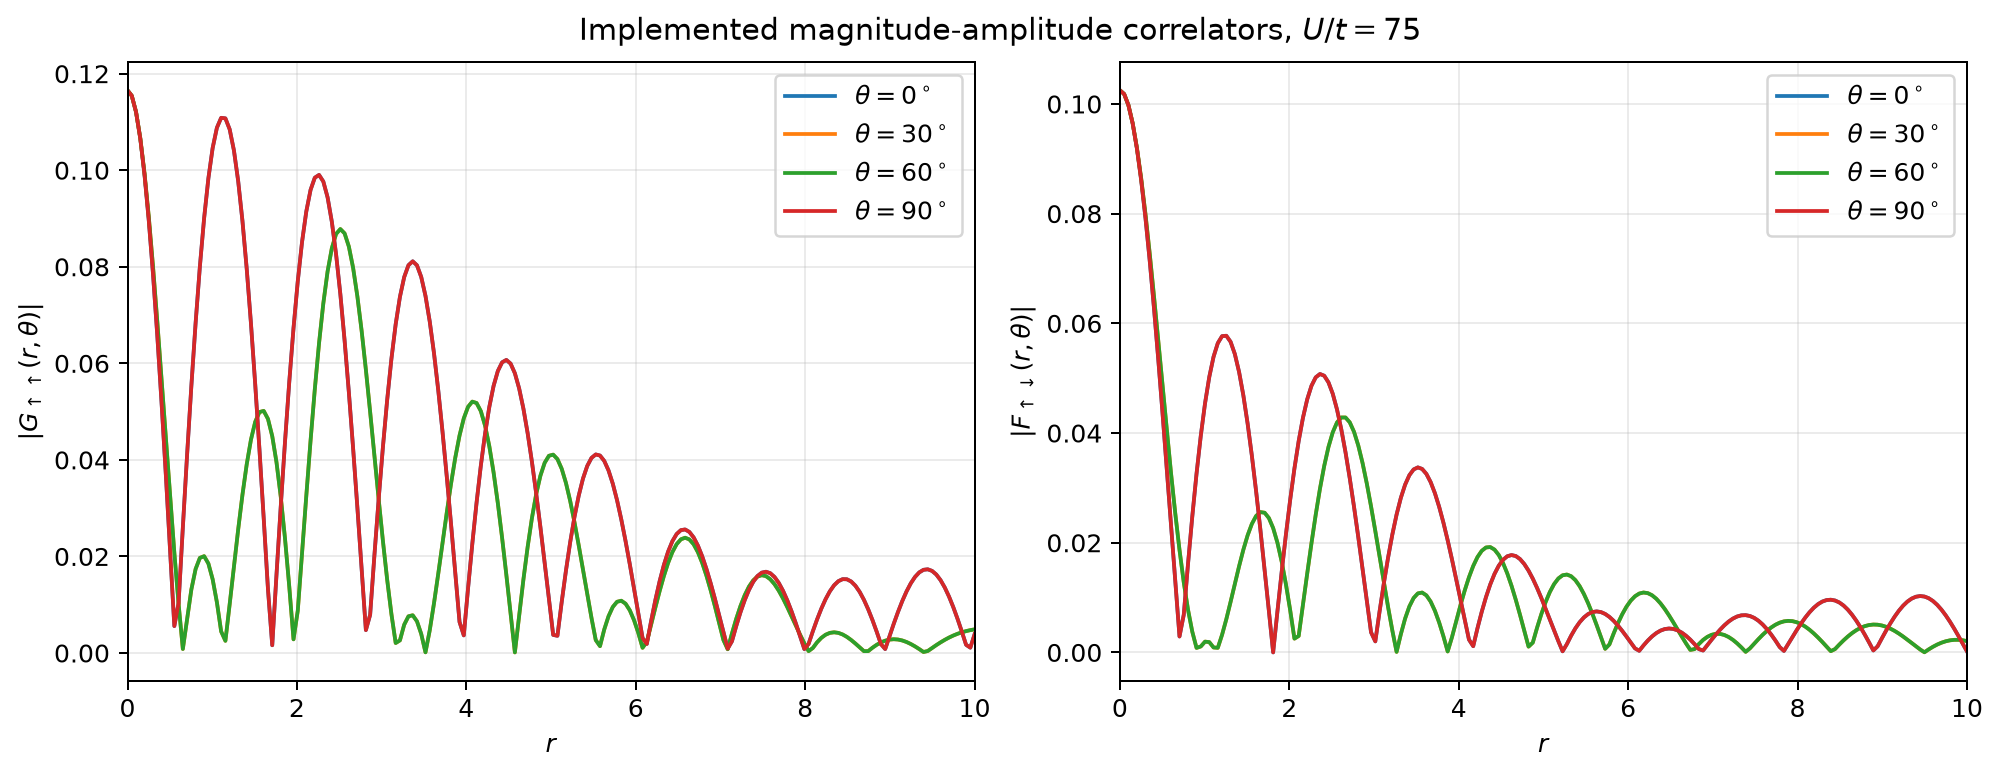
\includegraphics[width=0.97\textwidth]
    {figs/greens_angular.png}
    \caption{
    Angular dependence of the implemented normal and anomalous Green's-function
    magnitudes at $U/t=75$ and the initial time. The left panel shows
    $|G_{\uparrow\uparrow}(r,\theta)|$, while the right panel shows
    $|F_{\uparrow\downarrow}(r,\theta)|$, for $\theta=0^\circ$, $30^\circ$,
    $60^\circ$, and $90^\circ$. Both correlation functions exhibit damped
    spatial oscillations with direction-dependent amplitudes. The overlapping
    curves for $0^\circ$ and $90^\circ$, and for $30^\circ$ and $60^\circ$,
    reflect the square-lattice symmetry. These curves were regenerated from
    the same magnitude-amplitude implementation used for the archived data.
    }
    \label{fig:greens_angular}
\end{figure*}

As shown in Fig.~\ref{fig:greens_angular}, both implemented Green's functions
display oscillatory behavior with an overall decrease in magnitude as the
electron separation increases. The comparison among different values of
$\theta$ reveals directional dependence inherited from the lattice and the
self-consistent solution. The symmetry-related directions
$\theta=0^\circ$ and $90^\circ$ produce identical profiles to numerical
precision, as do $\theta=30^\circ$ and $60^\circ$.

A second point concerns the phase structure of the Green's functions.
Because $\epsilon_{ks}$ and the coherence amplitudes are even functions of
$\mathbf{k}$ on the square lattice, integration over the inversion-symmetric
Brillouin zone eliminates the odd contribution proportional to
$\sin(\mathbf{k}\cdot\mathbf{r})$. Consequently, the Green's functions may
be written as
%
\begin{equation}
G_{\uparrow\uparrow}(\mathbf{r})
=
-iA(\mathbf{r}),
\qquad
F_{\uparrow\downarrow}(\mathbf{r})
=
-iB(\mathbf{r}),
\label{eq:GF_imaginary}
\end{equation}
%
where $A(\mathbf{r})$ and $B(\mathbf{r})$ are real functions. For the signed
construction, we define the normalized correlation functions as
%
\begin{equation}
g(\mathbf{r})
=
\operatorname{Re}
\left[
\frac{G_{\uparrow\uparrow}(\mathbf{r})}
     {G_{\uparrow\uparrow}(\mathbf{0})}
\right],
\qquad
f(\mathbf{r})
=
\operatorname{Re}
\left[
\frac{F_{\uparrow\downarrow}(\mathbf{r})}
     {G_{\uparrow\uparrow}(\mathbf{0})}
\right].
\label{eq:normalized_GF}
\end{equation}
%
These normalized quantities are real in the continuum inversion-symmetric
limit. A finite momentum grid can leave a small residual imaginary component,
which is discarded by the real-part reduction.

The current numerical density-matrix builder instead uses
$|G(\mathbf r)|/|G(\mathbf0)|$ and $|F(\mathbf r)|/|G(\mathbf0)|$.
This distinction requires a precise qualification. The density matrix in
Eq.~\eqref{eq:density_matrix} contains only $g^2$ and $f^2$; consequently,
taking the absolute value of an already real normalized ratio does not change
that matrix in exact arithmetic. The physically consequential loss of sign
occurs if the sign of $\Delta_{ks}$ is discarded \emph{before} the
Brillouin-zone sum, as in the unsigned-amplitude implementation described
above. It is therefore incorrect to attribute the difference between the two
constructions merely to taking an absolute value after integration.

\subsection{Two-spin density matrix}
\label{sec:density_matrix}

The spatial correlations encoded in the normal and anomalous Green's
functions can be used to construct the reduced spin density matrix of
two electrons separated by $\mathbf{r}$~\cite{Oh2005}. In the basis
%
\begin{equation}
\{
|\uparrow\uparrow\rangle,
|\uparrow\downarrow\rangle,
|\downarrow\uparrow\rangle,
|\downarrow\downarrow\rangle
\},
\end{equation}
%
the resulting two-spin state takes the X-state form
%
\begin{equation}
\rho(\mathbf{r})
=
\frac{1}{\mathcal{N}}
\begin{pmatrix}
1-g^2 & 0 & 0 & 0 \\
0 & 1+f^2 & -(g^2+f^2) & 0 \\
0 & -(g^2+f^2) & 1+f^2 & 0 \\
0 & 0 & 0 & 1-g^2
\end{pmatrix},
\label{eq:density_matrix}
\end{equation}
%
where, for compactness, $g\equiv g(\mathbf{r})$ and
$f\equiv f(\mathbf{r})$ denote the normalized normal and anomalous
Green's functions defined in Eq.~\eqref{eq:normalized_GF}. The
normalization factor is
%
\begin{equation}
\mathcal{N}
=
4-2g^2+2f^2,
\label{eq:density_normalization}
\end{equation}
%
which ensures $\mathrm{Tr}\,\rho(\mathbf{r})=1$.

The X structure of Eq.~\eqref{eq:density_matrix} reflects the fact
that, for the present correlation functions, the nonvanishing
off-diagonal coherence occurs between the opposite-spin states
$|\uparrow\downarrow\rangle$ and
$|\downarrow\uparrow\rangle$. The quantity $g(\mathbf{r})$
describes the contribution associated with normal single-particle
correlations, whereas $f(\mathbf{r})$ contains the contribution
arising from superconducting pairing. Consequently, the spatial
dependence of the microscopic Green's functions is transferred
directly to the populations and coherences of the reduced two-spin
state.

Equation~\eqref{eq:density_matrix} can equivalently be written in
Werner-state form,
%
\begin{equation}
\rho(\mathbf{r})
=
\frac{1-p}{4}\mathbb{I}_{4}
+
p\,|\Psi^{-}\rangle\langle\Psi^{-}|,
\label{eq:werner_state}
\end{equation}
%
where
%
\begin{equation}
|\Psi^{-}\rangle
=
\frac{1}{\sqrt{2}}
\left(
|\uparrow\downarrow\rangle
-
|\downarrow\uparrow\rangle
\right)
\end{equation}
%
is the spin-singlet Bell state and
%
\begin{equation}
p(\mathbf{r})
=
\frac{f^2+g^2}
     {2+f^2-g^2}.
\label{eq:werner_parameter}
\end{equation}
%
Thus, the parameter $p(\mathbf{r})$ provides a direct connection
between the microscopic superconducting correlations and the
singlet content of the two-electron spin state. As the separation
between the electrons changes, the oscillatory behavior of
$g(\mathbf{r})$ and $f(\mathbf{r})$ modifies $p(\mathbf{r})$ and,
therefore, the amount of spin entanglement available in the reduced
state. In particular, $g(\mathbf0)=1$ implies $p(\mathbf0)=1$, so the
implemented zero-separation state is the pure singlet independently of
$f(\mathbf0)$.

The eigenvalues of the Werner state are
%
\begin{equation}
\lambda_{\mathrm{s}}
=
\frac{1+3p}{4},
\qquad
\lambda_{\mathrm{t}}
=
\frac{1-p}{4},
\label{eq:werner_eigenvalues}
\end{equation}
%
where $\lambda_{\mathrm{s}}$ corresponds to the singlet component
and $\lambda_{\mathrm{t}}$ is threefold degenerate for the triplet
subspace. These eigenvalues provide a convenient check of the
positivity of the reduced density matrix.

For a Werner state, the concurrence has the closed form
%
\begin{equation}
C(\mathbf{r})
=
\max
\left\{
0,
\frac{3p(\mathbf{r})-1}{2}
\right\},
\label{eq:werner_concurrence}
\end{equation}
%
showing that the state is entangled when $p>1/3$. The numerical routine
evaluates the X-state reduction of the Wootters concurrence for two-qubit
states~\cite{Wootters1998}. For the initial matrix structure in
Eq.~\eqref{eq:density_matrix}, this expression reduces identically to
Eq.~\eqref{eq:werner_concurrence}; the independent amplitude-damping map
preserves the X-state structure required by the numerical formula.

\subsection{Open-system evolution}
\label{sec:open_system}

For independent reservoirs, the two-qubit state evolves through
local Kraus maps according to
%
\begin{equation}
\rho(t)
=
\sum_{\alpha,\beta}
\left(
K_{\alpha}^{A}\otimes K_{\beta}^{B}
\right)
\rho(0)
\left(
K_{\alpha}^{A}\otimes K_{\beta}^{B}
\right)^{\dagger}.
\label{eq:kraus_evolution}
\end{equation}
%
Here, $K_{\alpha}^{A}$ and $K_{\beta}^{B}$ denote the single-qubit
Kraus operators associated with the reservoirs coupled to qubits
$A$ and $B$, respectively. The numerical implementation allows the
two reservoirs to have different coupling and memory parameters,
although identical parameters are used when the two environments
are chosen to be equivalent. All six archived figures analyzed below
use independent, equivalent amplitude-damping reservoirs.

For the non-Markovian amplitude-damping channel, the single-qubit
Kraus operators are
%
\begin{equation}
K_{0}(t)
=
\begin{pmatrix}
1 & 0 \\
0 & \sqrt{p(t)}
\end{pmatrix},
\qquad
K_{1}(t)
=
\begin{pmatrix}
0 & \sqrt{1-p(t)} \\
0 & 0
\end{pmatrix},
\label{eq:AD_kraus}
\end{equation}
%
where $p(t)$ is the excited-state survival probability. The lowercase
$\gamma$ is the system--reservoir coupling strength, whereas the uppercase
$\Gamma$ is the reservoir memory rate; they are not interchangeable.
For a Lorentzian reservoir in the oscillatory regime, the survival
probability is
%
\begin{equation}
p(t)
=
e^{-\Gamma t}
\left[
\cos\left(\frac{dt}{2}\right)
+
\frac{\Gamma}{d}
\sin\left(\frac{dt}{2}\right)
\right]^2,
\label{eq:AD_probability}
\end{equation}
%
with
%
\begin{equation}
d
=
\sqrt{2\gamma\Gamma-\Gamma^2}.
\label{eq:d_parameter}
\end{equation}
%
The oscillatory regime corresponds to $2\gamma>\Gamma$, for which $d$
is real. Both amplitude-damping regimes presented below satisfy this
condition.

For completeness, the exact continuation of Eq.~\eqref{eq:AD_probability}
to the overdamped regime, $2\gamma\leq\Gamma$, is obtained by defining
%
\begin{equation}
\tilde d
=
\sqrt{\Gamma^2-2\gamma\Gamma},
\end{equation}
%
so that
%
\begin{equation}
p(t)
=
e^{-\Gamma t}
\left[
\cosh\left(\frac{\tilde d t}{2}\right)
+
\frac{\Gamma}{\tilde d}
\sinh\left(\frac{\tilde d t}{2}\right)
\right]^2.
\label{eq:AD_probability_overdamped}
\end{equation}
%
This continuation is present in the standalone fidelity routine. The main
concurrence and Holevo evolution routines instead use a critically damped
expression outside the oscillatory regime; this discrepancy does not affect
any underdamped result reported here, but it must be resolved before an
overdamped study is undertaken.

An independent colored-dephasing channel is also implemented. Its
coherence-retention factor is
%
\begin{equation}
q(t)
=
\exp
\left[
-\frac{\gamma}{2}
\left(
t+
\frac{e^{-\Gamma t}-1}{\Gamma}
\right)
\right],
\label{eq:dephasing_factor}
\end{equation}
%
with the corresponding Kraus operators
%
\begin{equation}
K_{0}(t)
=
\begin{pmatrix}
1 & 0 \\
0 & q(t)
\end{pmatrix},
\qquad
K_{1}(t)
=
\begin{pmatrix}
0 & 0 \\
0 & \sqrt{1-q^2(t)}
\end{pmatrix}.
\label{eq:dephasing_kraus}
\end{equation}
%
These operators satisfy the completeness relation
%
\begin{equation}
\sum_{\alpha}
K_{\alpha}^{\dagger}K_{\alpha}
=
\mathbb{I},
\end{equation}
%
ensuring a trace-preserving quantum channel.

A collective-dephasing map is also available in the numerical
implementation. In the present work, however, all reported results
are obtained using independent reservoirs, so that the environmental
action on the two qubits is described by the local map in
Eq.~\eqref{eq:kraus_evolution}.

\subsection{Fidelity, teleportation, and Pauli-ensemble Holevo information}
\label{sec:information_measures}

The fidelity module uses the squared Uhlmann convention
\begin{equation}
\mathcal F_{\mathrm U}(\rho,\sigma)
=
\left[
\operatorname{Tr}
\sqrt{\sqrt{\rho}\,\sigma\,\sqrt{\rho}}
\right]^2.
\label{eq:uhlmann}
\end{equation}
Two references are calculated separately. The initial-state fidelity is
\begin{equation}
\mathcal F_{\mathrm i}(\mathbf r,t)
=
\mathcal F_{\mathrm U}\!\left[\rho(\mathbf r,t),\rho(\mathbf r,0)\right],
\end{equation}
which satisfies $\mathcal F_{\mathrm i}(\mathbf r,0)=1$ by construction.
The singlet-referenced fidelity is
\begin{equation}
\mathcal F_{\Psi^-}(\mathbf r,t)
=
\mathcal F_{\mathrm U}\!\left[\rho(\mathbf r,t),
|\Psi^-\rangle\langle\Psi^-|\right].
\end{equation}
Because the reference is pure, Eq.~\eqref{eq:uhlmann} reduces exactly to
\begin{equation}
\mathcal F_{\Psi^-}(\mathbf r,t)
=
\langle\Psi^-|\rho(\mathbf r,t)|\Psi^-\rangle
\equiv F_{\mathrm s}(\mathbf r,t),
\label{eq:singlet_fidelity}
\end{equation}
where $F_{\mathrm s}$ is the singlet fraction implemented in the observable
module. For the initial Werner state,
$F_{\mathrm s}(\mathbf r,0)=(1+3p(\mathbf r))/4$.

Neither $\mathcal F_{\mathrm i}$ nor $F_{\mathrm s}$ should be identified
without further analysis with operational teleportation performance. The
latter depends on the fully entangled fraction
\begin{equation}
\mathfrak f(\rho)=\max_{\mathcal B}\langle\mathcal B|\rho|\mathcal B\rangle,
\end{equation}
where the maximum is over the Bell basis after the local optimization
appropriate to the teleportation protocol. For a qubit resource, the optimized
average teleportation fidelity obeys
$\overline{\mathcal F}_{\mathrm{tel}}=(2\mathfrak f+1)/3$~\cite{Horodecki1999}.
For the initial Werner state, $\mathfrak f=F_{\mathrm s}$ because the singlet
eigenvalue in Eq.~\eqref{eq:werner_eigenvalues} is the largest Bell weight.
No corresponding local optimization is performed for the evolved states in
the repository. We therefore do not assign teleportation thresholds to the
singlet-fidelity plots below, and the horizontal lines drawn by the plotting
routine are visual guides only.

For dense coding, the implemented encoding ensemble consists of four
equiprobable messages prepared by
\begin{equation}
\rho_i=(\mathcal U_i\otimes I_B)\rho_{AB}
       (\mathcal U_i\otimes I_B)^\dagger,
\qquad
\mathcal U_i\in\{I,\sigma_x,\sigma_y,\sigma_z\},
\end{equation}
with $p_i=1/4$. Here $\mathcal U_i$ denotes an encoding unitary, not the
Hubbard interaction $U$. The averaged encoded state is
$\bar\rho_{AB}=\sum_i\rho_i/4$, and the code calculates
\begin{equation}
\chi_{\mathrm P}
=
S_2(\bar\rho_{AB})-S_2(\rho_{AB}),
\qquad
S_2(\rho)=-\operatorname{Tr}(\rho\log_2\rho).
\label{eq:holevo_definition}
\end{equation}
The subscript P emphasizes the specified Pauli ensemble. The unitaries act on
subsystem $A$ after the open-system evolution; no additional encoding or
transmission noise is applied by this calculation.

The equal-probability Pauli twirl permits an exact simplification. Writing
$\rho_{AB}$ in $2\times2$ blocks with respect to subsystem $A$, the four
encodings remove the off-diagonal $A$ blocks and equalize the two diagonal
blocks. Hence
\begin{equation}
\bar\rho_{AB}
=
\frac{I_A}{2}\otimes\rho_B,
\qquad
\rho_B=\operatorname{Tr}_A\rho_{AB},
\label{eq:pauli_average}
\end{equation}
and therefore
\begin{equation}
\chi_{\mathrm P}
=
1+S_2(\rho_B)-S_2(\rho_{AB}).
\label{eq:holevo_entropy}
\end{equation}
Equation~\eqref{eq:holevo_entropy} was also checked directly against the
four-unitary implementation. Strong subadditivity gives
$0\leq\chi_{\mathrm P}\leq2$ bits for a two-qubit state. This is the Holevo
quantity of the specified ensemble and the dense-coding capacity when the
protocol is restricted to this encoding with ideal subsequent transmission
and the corresponding asymptotic joint decoding~\cite{Bruss2004}. It is not,
without those conditions, a general optimization over all encodings or a
one-shot accessible-information result. The value $\chi_{\mathrm P}=1$ bit is
the one-qubit classical benchmark; values above one bit indicate a quantum
advantage for this protocol.

A useful limiting check follows from Eq.~\eqref{eq:holevo_entropy}. Independent
amplitude damping drives both qubits to their common ground state as
$p(t)\to0$. The resulting pure product state has $S_2(\rho_{AB})=S_2(\rho_B)=0$
and therefore $\chi_{\mathrm P}\to1$, even though its concurrence and singlet
fraction both vanish. The three quantities consequently need not exhibit the
same dynamics.

\subsection{Numerical grids and validation}
\label{sec:validation}

The archived $\gamma=1.5$ data use $\gamma_A=\gamma_B=1.5$,
$\Gamma_A=\Gamma_B=0.1$, $200$ radial points on $0\leq r\leq10$, $261$ times on
$0\leq t\leq80$, and $\theta=0^\circ,15^\circ,\ldots,90^\circ$. The archived
$\gamma=4.5$ data use $\gamma_A=\gamma_B=4.5$, $\Gamma_A=\Gamma_B=0.01$, the
same radial and angular grids, and $161$ time points on the same time interval.
The primary angular slice is $45^\circ$ in the first regime and $0^\circ$ in the
second. These regimes are analyzed separately below.

Recomputing the initial Green's functions at $U/t=75$ with the fixed parameters
above reproduces the archived $\gamma=1.5$ arrays to $1.6\times10^{-16}$ maximum
absolute error and the $\gamma=4.5$ arrays to $1.3\times10^{-12}$. This
numerical agreement establishes the model settings of the archived runs, whose
NPZ files do not themselves contain a complete parameter record. The initial
states are Hermitian and positive semidefinite with unit trace to the tested
tolerance. Reconstructed concurrence and singlet-fraction arrays agree with the
archived angular data to $2.3\times10^{-15}$; the singlet-referenced fidelity
agrees to $1.5\times10^{-8}$. The entropy-based Holevo reconstruction agrees
with the archived four-Pauli calculation to $3.7\times10^{-11}$. Additional
direct tests of Eq.~\eqref{eq:kraus_evolution} gave unit trace and Hermiticity,
with no negative eigenvalues at the sampled points. The small differences in
fidelity are consistent with the separate eigensystem implementation and its
eigenvalue clipping.

The separate lower-interaction density study uses the corrected equal-time
normal weight $v_{\mathbf k}^2$ and signed anomalous weight
$\Delta_{\mathbf k}/(2E_{\mathbf k})$, with the mean of the two degenerate
helicity contributions. It varies $n$ over
$0.5,0.75,1.0,1.25,1.5,1.75,1.875$ at fixed $U/t=15$ and $25$,
$\Delta_t/t=4.5$, $V_{\mathrm{SO}}=0$, and $T=0$. Production results use
$N_k=400$, with $N_k=100,200,400,800$ convergence comparisons and six
independent solver seeds at $N_k=100$. Continuous radial curves are evaluated
at seven angles. Exact lattice resources are separately evaluated at ten
integer vectors from $(1,0)$ through $(4,0)$, rather than assigned from a
continuous radial grid. The irrelevant global gap sign is fixed by choosing
$\Delta_S\leq0$. Small residuals and seed/mesh reproducibility establish
stationary numerical branches, not global free-energy minima.

For the resulting initial Werner state, the fixed singlet-reference protocol
and local-unitary-optimized standard protocol have the same average fidelity,
\begin{equation}
\overline{\mathcal F}_{\mathrm{tel}}=\frac{1+p}{2},
\qquad
F_{\mathrm s}=\mathfrak f=\frac{1+3p}{4}.
\label{eq:werner_tel_lowerU}
\end{equation}
Consequently $\overline{\mathcal F}_{\mathrm{tel}}>2/3$ exactly when $p>1/3$
and $C>0$. These operational identities are applied only to the new initial
Werner resources, not retroactively to the legacy evolved X states.

\section{Results and Discussion}

\subsection{Spatial concurrence and interaction dependence}
\label{sec:concurrence_results}

We first examine the spatial structure of the entanglement contained in the
two-electron state before the open-system evolution is applied. As shown in
Sec.~\ref{sec:density_matrix}, the reduced two-spin density matrix can be
written in Werner form with
%
\begin{equation}
p(\mathbf r)
=
\frac{f^2(\mathbf r)+g^2(\mathbf r)}
     {2+f^2(\mathbf r)-g^2(\mathbf r)}.
\label{eq:p_results}
\end{equation}
%
The corresponding concurrence therefore takes the closed form
%
\begin{equation}
C(\mathbf r)
=
\max
\left\{
0,
\frac{3p(\mathbf r)-1}{2}
\right\},
\label{eq:concurrence_results}
\end{equation}
%
so that the two-spin state is entangled only when
$p(\mathbf r)>1/3$. Since both $g(\mathbf r)$ and $f(\mathbf r)$
are determined by the microscopic normal and anomalous Green's functions,
Eq.~\eqref{eq:concurrence_results} directly connects the spatial
entanglement to the underlying superconducting correlations.

To investigate how this entanglement is modified by the interaction strength
and lattice direction, Fig.~\ref{fig:concurrence_U_theta} shows
$C(r,\theta,0)$ for $U/t=20$, $44$, $79$, and $115$ and for the representative
directions $\theta=0^\circ$, $30^\circ$, $60^\circ$, and $90^\circ$. These
solutions passed the same residual and positivity checks. A previously listed
$U/t=150$ case is not included because the tested solver outputs did not meet
the residual criterion and therefore cannot support a converged numerical
claim.
%
\begin{figure*}[t]
    \centering
    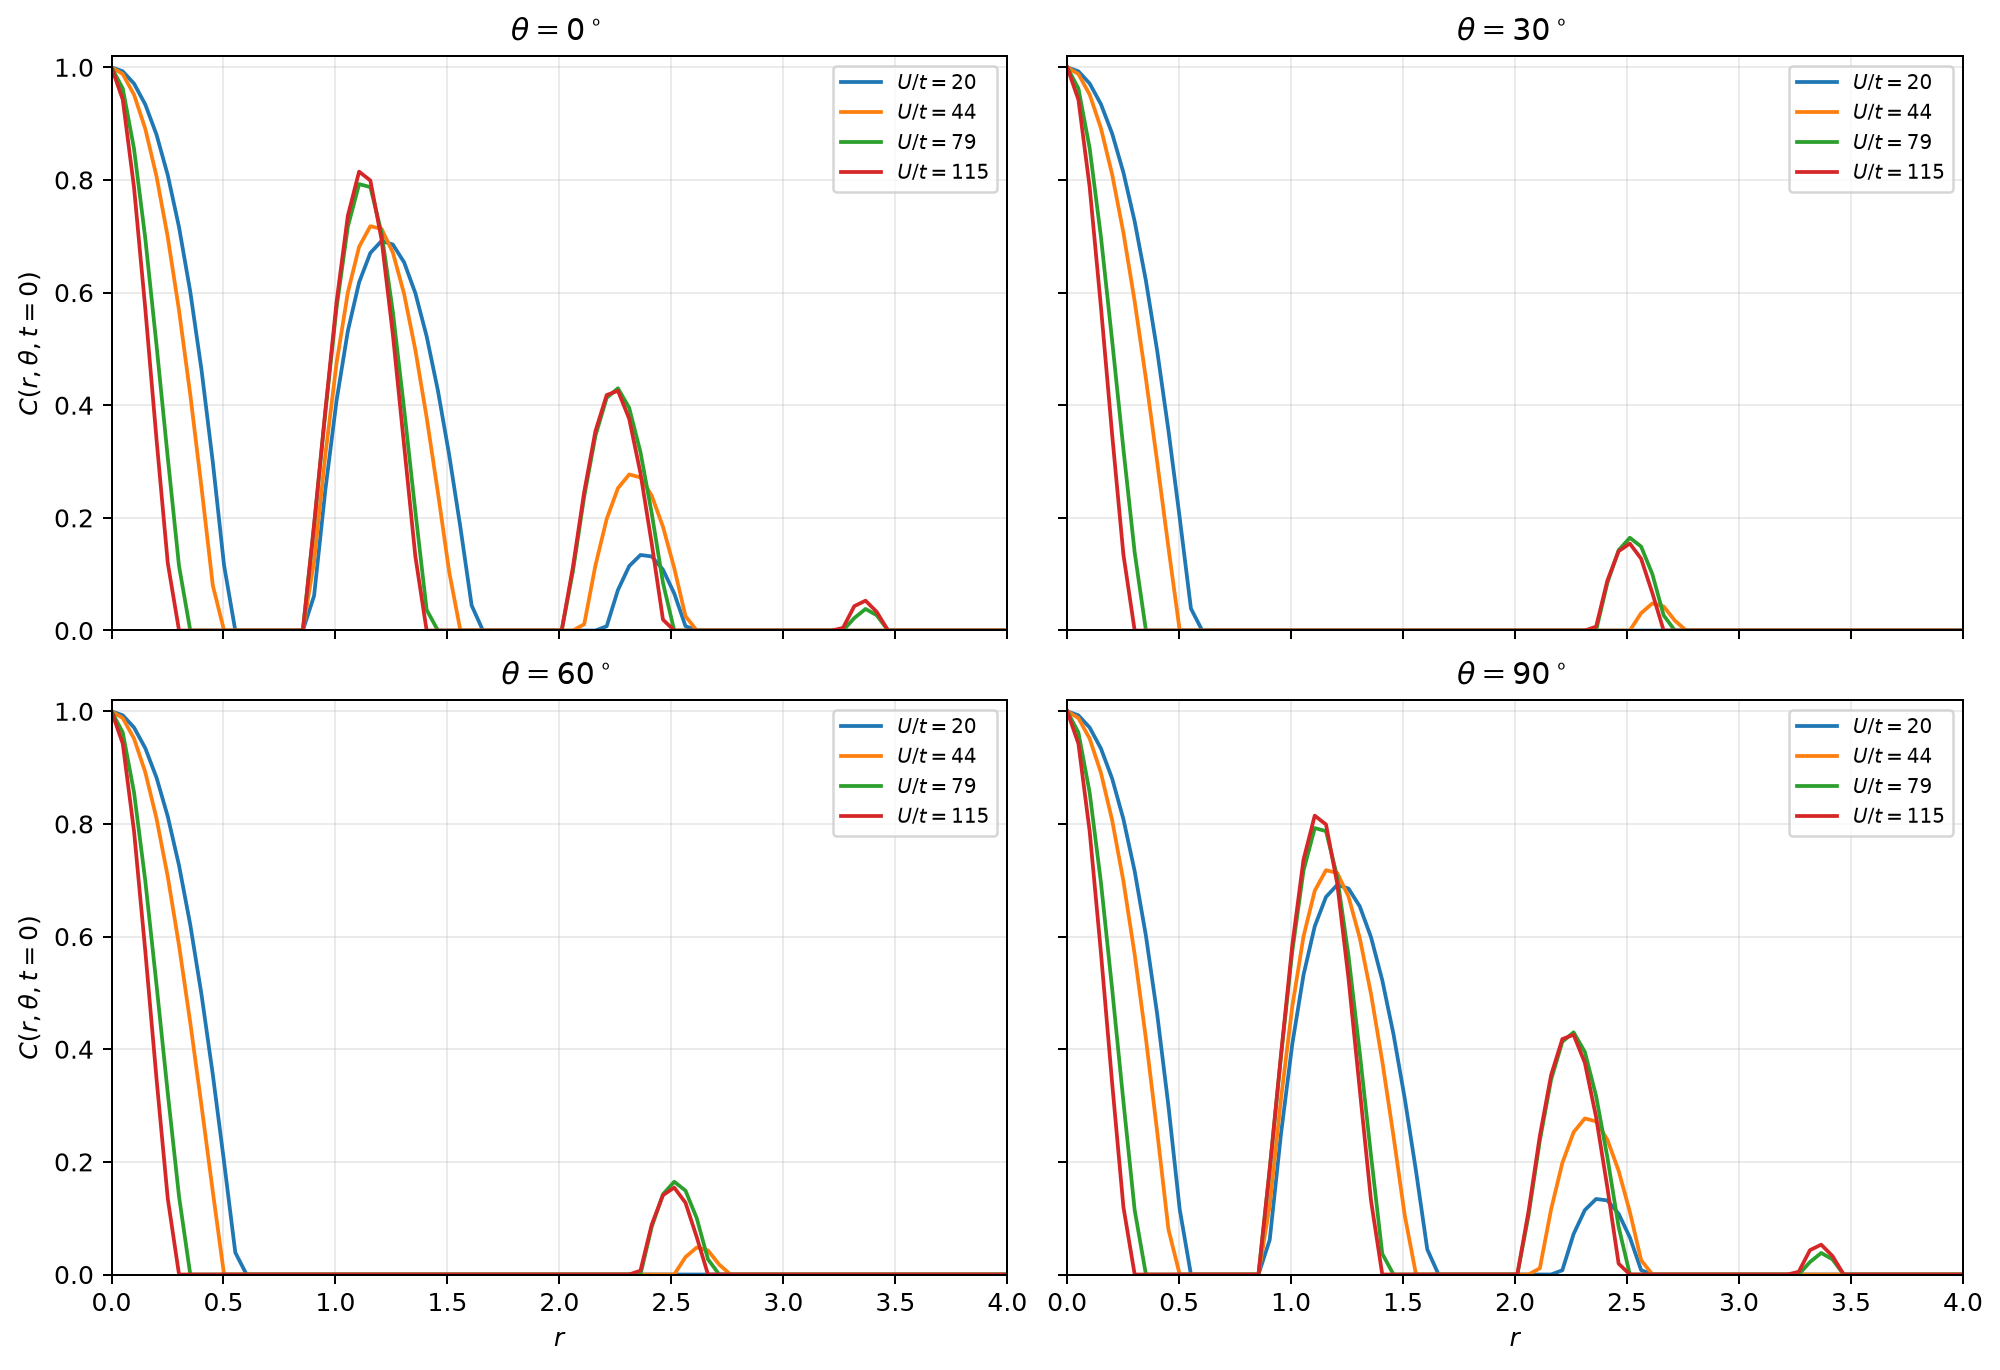
\includegraphics[width=\textwidth]
    {figs/concurrence_U_theta.png}
    \caption{
    Initial spatial dependence of the concurrence $C(r,\theta,0)$ for
    $U/t=20$, $44$, $79$, and $115$, evaluated along
    $\theta=0^\circ$, $30^\circ$, $60^\circ$, and $90^\circ$.
    The concurrence equals unity at $r=0$ and decreases to zero at a
    $U$-dependent finite separation. Along the lattice-axis directions,
    additional finite-$r$ entangled regions appear because of the oscillatory
    spatial dependence of the implemented Green's functions. Off-axis revival
    windows are weaker and occur at different separations. Increasing $U$
    shortens the first entangled interval in these examples but does not
    suppress every finite-$r$ revival amplitude.
    }
    \label{fig:concurrence_U_theta}
\end{figure*}

Several features are evident from Fig.~\ref{fig:concurrence_U_theta}.
At $r=0$, the concurrence is unity for all interaction strengths, as required
by $p(\mathbf0)=1$. As the electrons are separated, $C$ decreases rapidly and
reaches zero at a finite distance. The precise location of this first
entanglement boundary depends on $U$, demonstrating that the interaction
modifies the real-space range over which the implemented superconducting
correlations support two-spin entanglement.

The interaction dependence is not a uniform suppression of the concurrence.
For the parameters considered here, the $U/t=20$ curve retains nonzero
concurrence to the largest separation within the first connected interval.
Increasing $U$ shifts this first zero toward smaller $r$. In the first axial
revival window around $r\simeq1.1$--$1.3$, however, the peak concurrence is
larger for $U/t=79$ and $115$ than for $U/t=20$. Thus the interaction changes
both the entanglement boundaries and the spatial oscillation amplitudes, and
no single ordering applies at every separation.

A pronounced directional dependence is also visible. For
$\theta=0^\circ$ and $90^\circ$, the concurrence reappears after the first
zero and forms additional entangled windows, including the first strong
revival and a second region around $r\simeq2.1$--$2.6$. These disconnected
regions are a direct consequence of the oscillatory real-space Green's
functions: when $p(r,\theta)$ falls below $1/3$ the state becomes separable,
while subsequent oscillations can drive it above the threshold again.

By contrast, the off-axis revival structure along $\theta=30^\circ$ and
$60^\circ$ is weaker and displaced to larger $r$ in the displayed interval.
The exact agreement between the $0^\circ$ and $90^\circ$ results, and between
the $30^\circ$ and $60^\circ$ results, reflects the square-lattice symmetry.
These are spatial revivals of the initial entanglement, not environmental
memory effects; the open-system time has not yet been introduced.

\subsection{Density and lower-interaction dependence of initial Werner resources}
\label{sec:lower_U_density}

The fixed-filling calculations above do not determine whether pairing or
normal exchange controls the finite-separation resource at other densities.
We therefore independently solved the self-consistent equations at seven
fillings for $U/t=15$ and $25$, using the corrected equal-time construction
and validation procedure described in Sec.~\ref{sec:validation}. Throughout
this subsection $\Delta_t/t=4.5$, $V_{\mathrm{SO}}=0$, and $T=0$.
Table~\ref{tab:low_U_solutions} reports the production self-consistent
solutions.

\begin{table*}[t]
\caption{\label{tab:low_U_solutions}
Self-consistent lower-interaction solutions at $N_k=400$. The gap gauge is
$\Delta_S\leq0$; reversing both gap signs leaves all resource magnitudes
unchanged. Energies are in units of $t$. The maximum residual over these 14
selected solutions is $6.28\times10^{-10}$, and the discrete occupations
reproduce the target fillings. These are stationary BdG branches, not proven
global thermodynamic ground states.}
\begin{ruledtabular}
\begin{tabular}{cccccc}
$U/t$ & $n$ & $\Delta_0/t$ & $\Delta_S/t$ & $\mu/t$ &
$\max_{\mathbf k}|\Delta_{\mathbf k}|/t$ \\
\colrule
15 & 0.500 & +0.181123 & -0.512376 & -1.443074 & 0.693499 \\
15 & 0.750 & +0.600845 & -2.393505 & -0.837215 & 2.994351 \\
15 & 1.000 & +0.686216 & -3.234806 & -0.309485 & 3.921022 \\
15 & 1.250 & +0.727005 & -3.572029 & +0.321745 & 4.299034 \\
15 & 1.500 & +0.757316 & -3.491605 & +1.310577 & 4.248920 \\
15 & 1.750 & +0.720193 & -2.904189 & +2.962452 & 3.624382 \\
15 & 1.875 & +0.601116 & -2.215107 & +4.137529 & 2.816223 \\
25 & 0.500 & 0 & 0 & -1.430404 & 0 \\
25 & 0.750 & 0 & 0 & -0.556922 & 0 \\
25 & 1.000 & +0.196566 & -1.854346 & -0.098078 & 2.050913 \\
25 & 1.250 & +0.231641 & -2.363357 & +0.393635 & 2.594998 \\
25 & 1.500 & +0.274079 & -2.561070 & +1.256200 & 2.835149 \\
25 & 1.750 & +0.296515 & -2.291915 & +2.696877 & 2.588431 \\
25 & 1.875 & +0.264617 & -1.798159 & +3.724770 & 2.062776 \\
\end{tabular}
\end{ruledtabular}
\end{table*}

At $U/t=15$, every sampled density has a nonzero-gap stationary solution.
This contrasts with the corrected $U/t=75$ density sweep, in which such
solutions were found only at $n=1.75$ and $1.875$. The absence of pairing at
low density is therefore interaction dependent, not a universal property of
the lattice model. At $U/t=25$, the production and finest meshes give zero
gap at $n=0.5$ and $0.75$, and nonzero gaps for $n\geq1$. A small solution at
$n=0.75,N_k=100$, with $\Delta_0/t=0.00278215$ and
$\Delta_S/t=-0.02034372$, disappears at $N_k=200,400,800$ and is accordingly
not presented as a robust paired state.

\begin{figure*}[t]
\centering
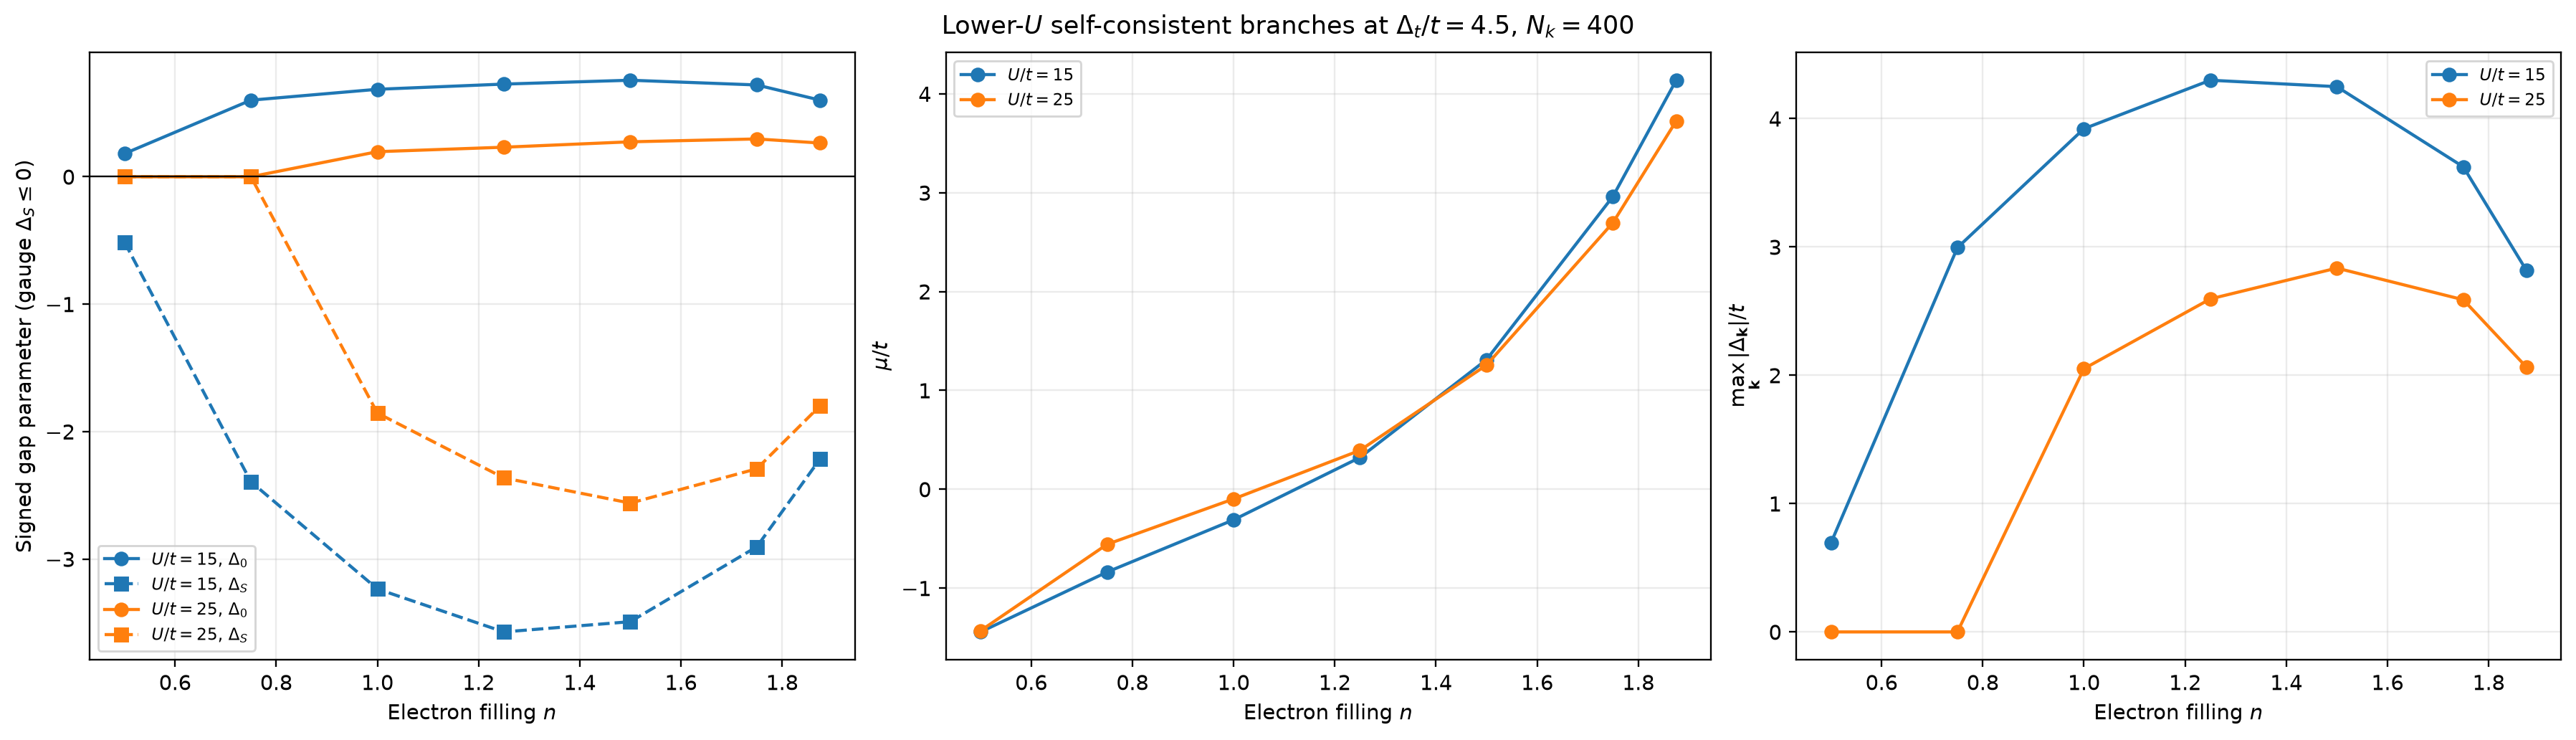
\includegraphics[width=\textwidth]{figs/low_U_density_bdg_solutions.png}
\caption{\label{fig:low_U_solutions}
Density dependence of the self-consistent gap parameters, chemical potential,
and maximum momentum-space gap at $U/t=15$ and $25$, using
$\Delta_t/t=4.5$, $V_{\mathrm{SO}}=0$, $T=0$, and $N_k=400$. The gap gauge is
$\Delta_S\leq0$. Large order parameters at $U/t=15$ should not be interpreted
through weak-coupling BCS estimates.}
\end{figure*}

Figure~\ref{fig:low_U_solutions} shows that the extended-$s$ component is
large at intermediate filling for $U/t=15$. The maximum momentum-space gap
reaches $4.299034t$ at $n=1.25$, so weak-coupling approximations are not
appropriate. Six independent seeds reproduce each accepted coarse-mesh root
after fixing the global gap gauge. This reproducibility does not establish
global thermodynamic stability or exclude competing orders.

The corresponding quantum-resource results are listed in
Table~\ref{tab:low_U_resources}. The continuous critical radius $r_c$ is the
first down-crossing of $p=1/3$ along $\theta=45^\circ$. It is a Fourier
interpolation of the lattice model, not an additional physical sub-lattice
detector location. In contrast, $p(a)$ and
$\overline{\mathcal F}_{\mathrm{tel}}(a)$ are evaluated exactly at the
nearest-neighbor vector $(1,0)$.

\begin{table*}[t]
\caption{\label{tab:low_U_resources}
Continuous-distance critical radii and exact nearest-neighbor resources for
the lower-interaction density sweep. The $45^\circ$ critical radii are shown
at $N_k=400$ and $800$. Exact-site quantities use $N_k=400$. Every tabulated
nearest-neighbor state has $C=0$; the same conclusion holds at the diagonal
$(1,1)$ and the other eight tested nonzero vectors.}
\begin{ruledtabular}
\begin{tabular}{ccccccc}
$U/t$ & $n$ & $r_c/a$ ($400$) & $r_c/a$ ($800$) & $f^2(a)$ & $p(a)$ &
$\overline{\mathcal F}_{\mathrm{tel}}(a)$ \\
\colrule
15 & 0.500 & 0.896729 & 0.900066 & 0.007581 & 0.268080 & 0.634040 \\
15 & 0.750 & 0.664634 & 0.665807 & 0.055339 & 0.130355 & 0.565177 \\
15 & 1.000 & 0.581330 & 0.581893 & 0.050471 & 0.075884 & 0.537942 \\
15 & 1.250 & 0.536287 & 0.536610 & 0.038341 & 0.046447 & 0.523224 \\
15 & 1.500 & 0.505851 & 0.506049 & 0.026540 & 0.026529 & 0.513264 \\
15 & 1.750 & 0.479129 & 0.479252 & 0.014815 & 0.011185 & 0.505593 \\
15 & 1.875 & 0.465440 & 0.465519 & 0.008027 & 0.005023 & 0.502512 \\
25 & 0.500 & 0.905807 & 0.906945 & 0 & 0.273016 & 0.636508 \\
25 & 0.750 & 0.735026 & 0.736053 & 0 & 0.154624 & 0.577312 \\
25 & 1.000 & 0.605579 & 0.606498 & 0.026865 & 0.084440 & 0.542220 \\
25 & 1.250 & 0.543882 & 0.544288 & 0.027418 & 0.050022 & 0.525011 \\
25 & 1.500 & 0.508550 & 0.508785 & 0.022864 & 0.027726 & 0.513863 \\
25 & 1.750 & 0.479927 & 0.480072 & 0.014182 & 0.011450 & 0.505725 \\
25 & 1.875 & 0.465810 & 0.465905 & 0.007915 & 0.005098 & 0.502549 \\
\end{tabular}
\end{ruledtabular}
\end{table*}

\begin{figure*}[t]
\centering
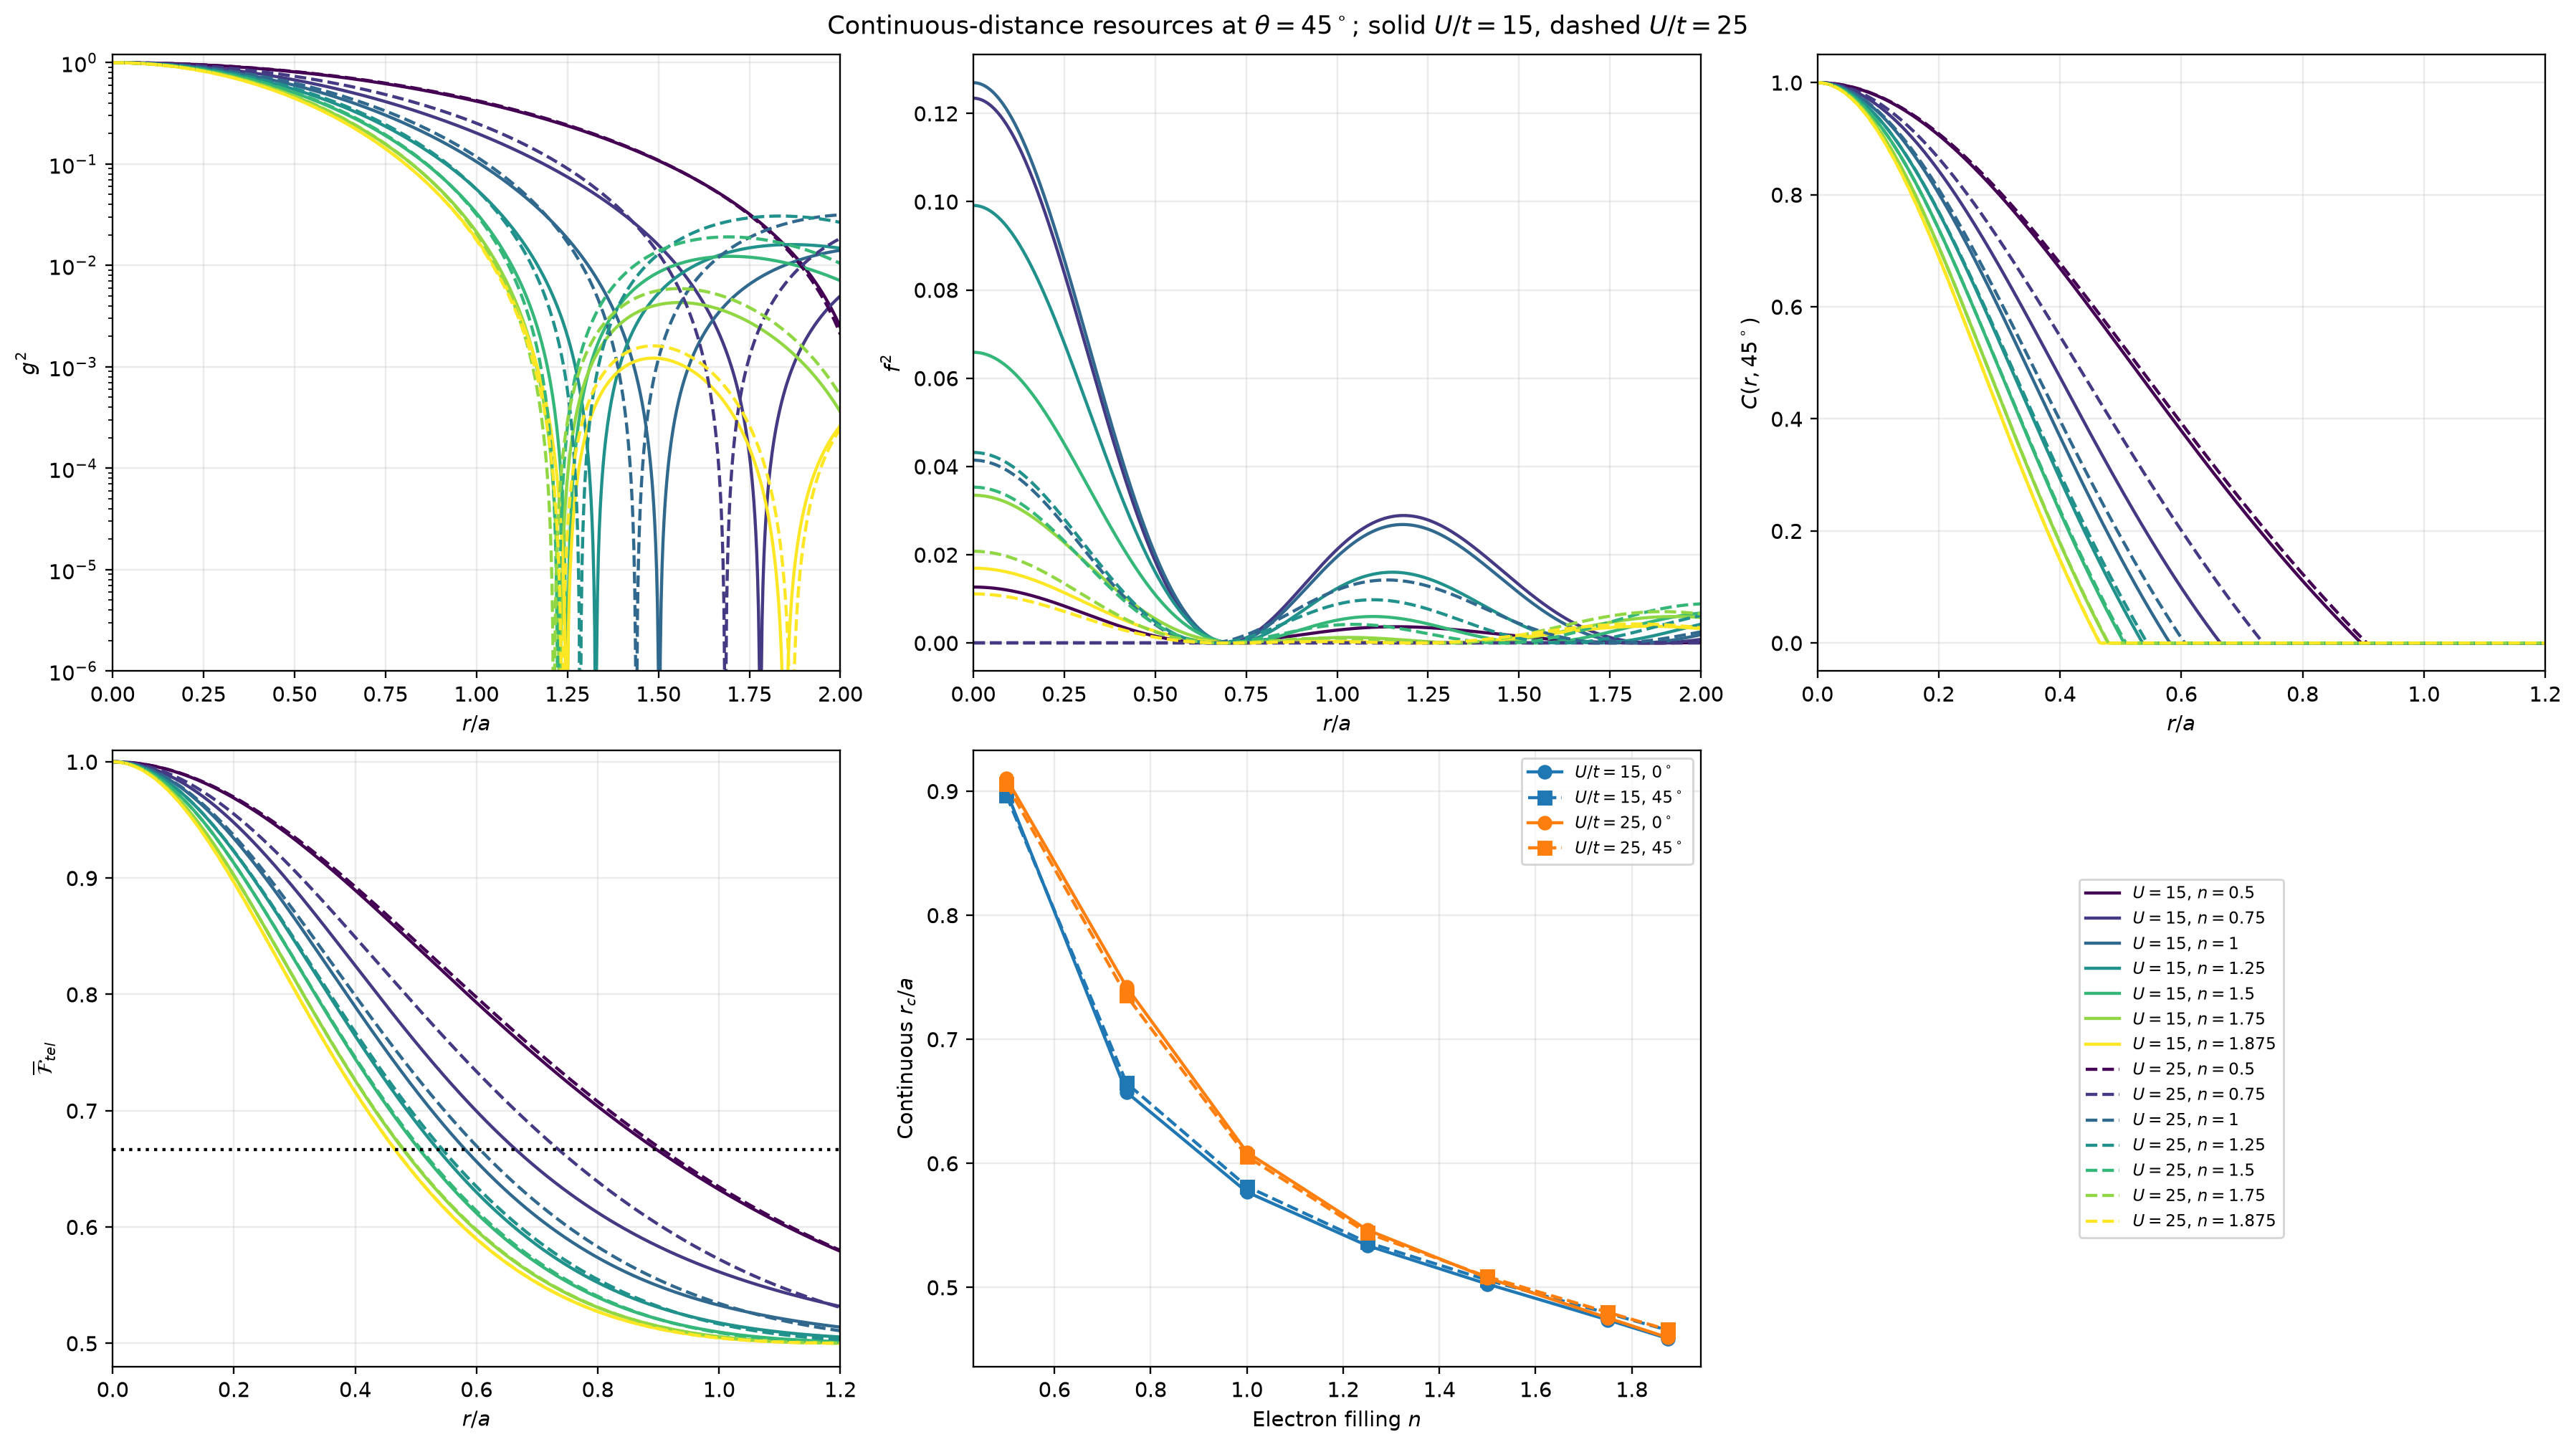
\includegraphics[width=\textwidth]{figs/low_U_density_resources.png}
\caption{\label{fig:low_U_resource_curves}
Continuous Fourier-interpolated resources at $U/t=15$ (solid) and $25$
(dashed), with $\Delta_t/t=4.5$ and $N_k=400$. Panels show normalized normal
and anomalous correlators, concurrence, average teleportation fidelity, and
the first $45^\circ$ critical radius. Concurrence is threshold-clipped even
when the underlying correlators continue to oscillate. Continuous curves must
be distinguished from the exact-site results in
Fig.~\ref{fig:low_U_exact_sites}.}
\end{figure*}

The larger anomalous correlations generated at lower $U$ do not produce an
operational finite-site advantage. For example, at $U/t=15,n=0.75$ the
nearest-neighbor anomalous weight is $f^2(a)=0.055339$, much larger than in
the corrected $U/t=75,n=1.875$ state. Nevertheless, $p(a)=0.130355$, far below
$1/3$. The reason is that the Werner threshold depends on $2g^2+f^2$, and
pairing also changes $v_{\mathbf k}^2$ and hence the normal exchange
correlation. At $45^\circ$, every nonzero-gap lower-$U$ production branch has
a shorter first continuous entanglement window than its same-filling
zero-gap reference, although pairing can increase $p(a)$ at the highest three
sampled fillings.

\begin{figure*}[t]
\centering
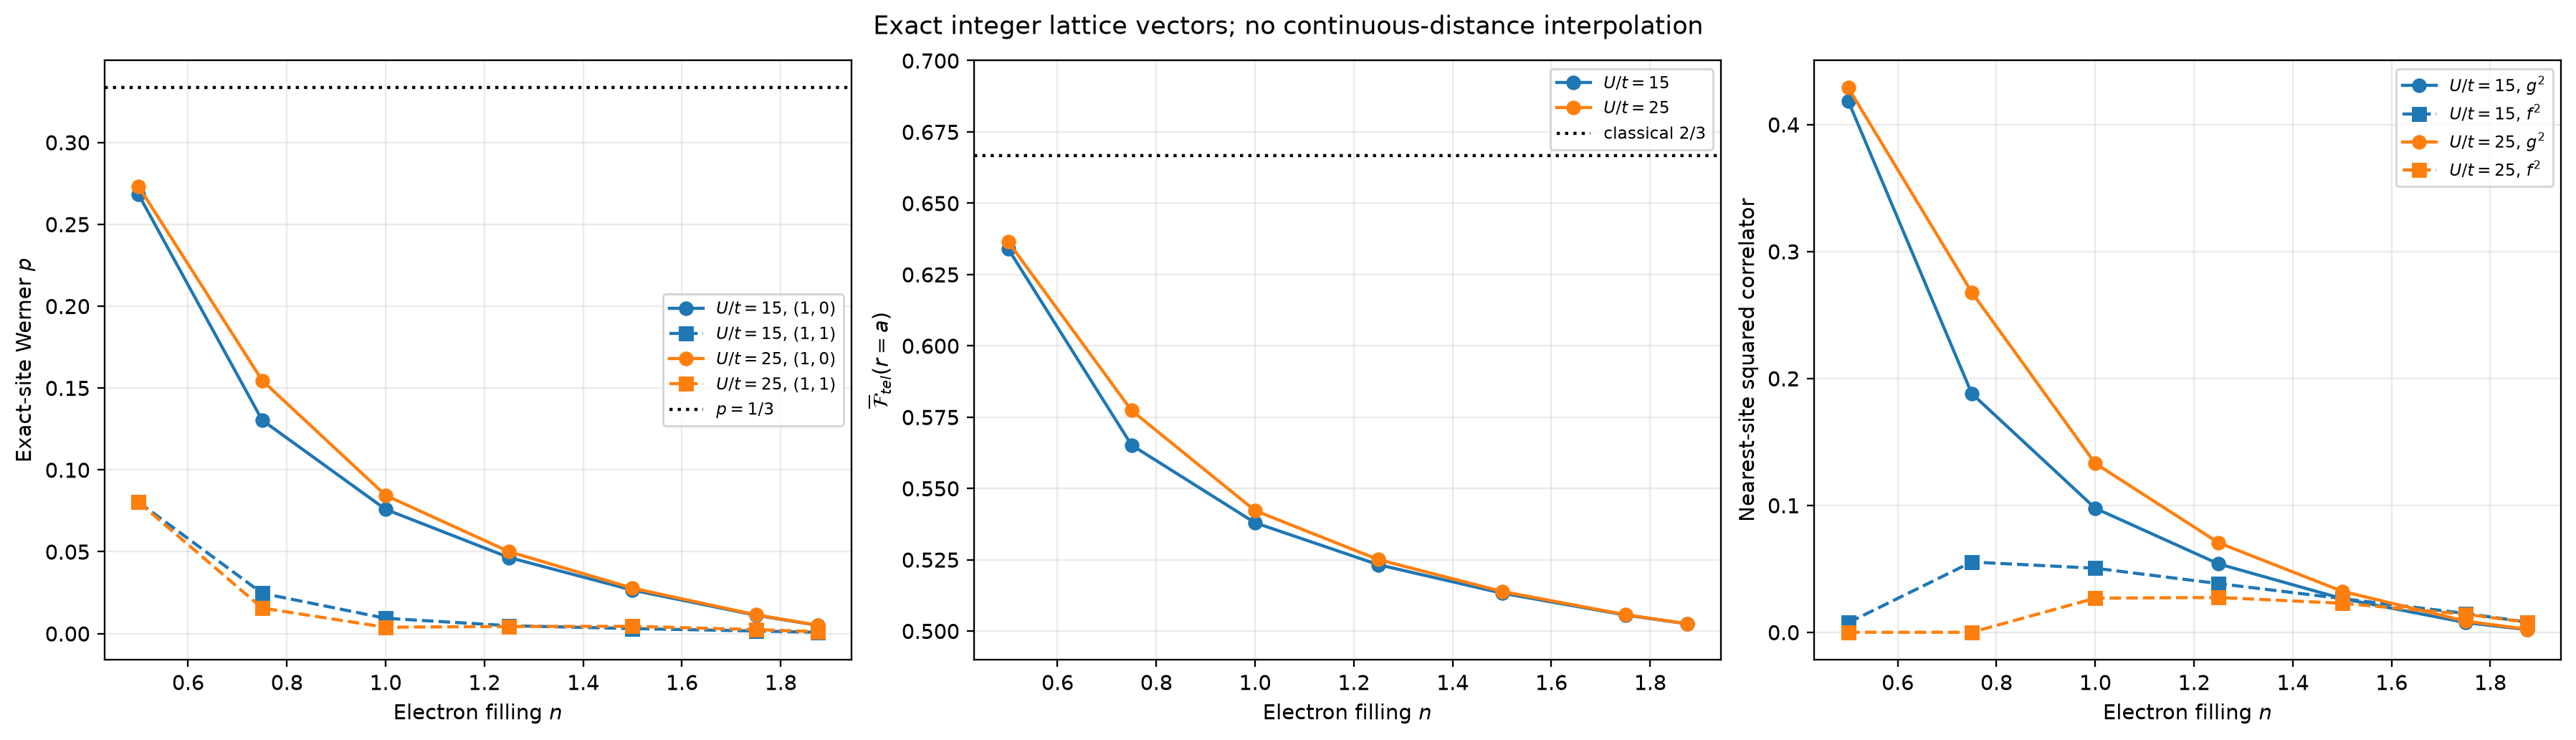
\includegraphics[width=\textwidth]{figs/low_U_density_lattice_sites.png}
\caption{\label{fig:low_U_exact_sites}
Exact integer-lattice-vector resources at $N_k=400$. Left: Werner parameter at
$(1,0)$ and $(1,1)$. Center: nearest-neighbor average teleportation fidelity.
Right: squared normal and anomalous correlators at $(1,0)$. None of the 140
production states obtained from two interactions, seven fillings, and ten
nonzero vectors crosses $p=1/3$ or $\overline{\mathcal F}_{\mathrm{tel}}=2/3$.
The same negative threshold result holds on all four momentum meshes.}
\end{figure*}

Figure~\ref{fig:low_U_exact_sites} demonstrates the central result: all 140
tested nonzero production resources have $C=0$. The strongest exact-site case
is the zero-gap $U/t=25,n=0.5,(1,0)$ state, with
$p=0.273016$ and $\overline{\mathcal F}_{\mathrm{tel}}=0.636508<2/3$.
Superconductivity is therefore not a logical prerequisite for defining the
conditional two-spin state: when $F=0$, normal exchange gives
$p=g^2/(2-g^2)$, which can still yield entanglement if $g^2>1/2$
\cite{Oh2004}. Conversely, a Cooper-pair anomalous function is not sufficient
for useful teleportation. In the present site-based model, neither mechanism
crosses the operational threshold at any tested nonzero lattice vector.

The $400\to800$ change in $r_c/a$ is below $0.00118$ except for
$U/t=15,n=0.5$, where it is $0.003337$ and the maximum gap changes from
$0.693499$ to $0.600171$. This slowly converging case is therefore not quoted
with continuum-limit precision; its nearest-neighbor $p$ changes only from
$0.268080$ to $0.270049$ and remains below threshold. Across all cases the
$400\to800$ nearest-site $p$ change is below $0.002$. No upward $p=1/3$
recrossing after the first loss was found at any of the seven sampled angles
out to $r=10a$ for either interaction.

The corrected initial-state study passed 64 independent artifact checks,
including filling and residual tests, seed reproducibility, Werner and
protocol identities, positivity, angular symmetries, and exact-site checks on
all meshes. Fixed and optimized protocol formulas were verified over 392
sampled states. These new results do not constitute a signed-versus-unsigned
regeneration of the legacy open-system dynamics considered below.

\subsection{Non-Markovian concurrence and singlet fidelity}
\label{sec:high_regime}

We now consider the regime $\gamma_A=\gamma_B=4.5$ and
$\Gamma_A=\Gamma_B=0.01$. Figure~\ref{fig:C_high_heatmap} shows the
concurrence along $\theta=0^\circ$. Entanglement is concentrated in separated
spatial islands at the initial time and in repeated temporal windows. Within
each temporal window the radial locations remain tied to the initial spatial
correlation profile, while the envelope weakens at later times. The repeated
windows are consistent with the oscillations of the exact survival probability
in Eq.~\eqref{eq:AD_probability}; no additional revival mechanism is required
to explain them.

\begin{figure*}[t]
    \centering
    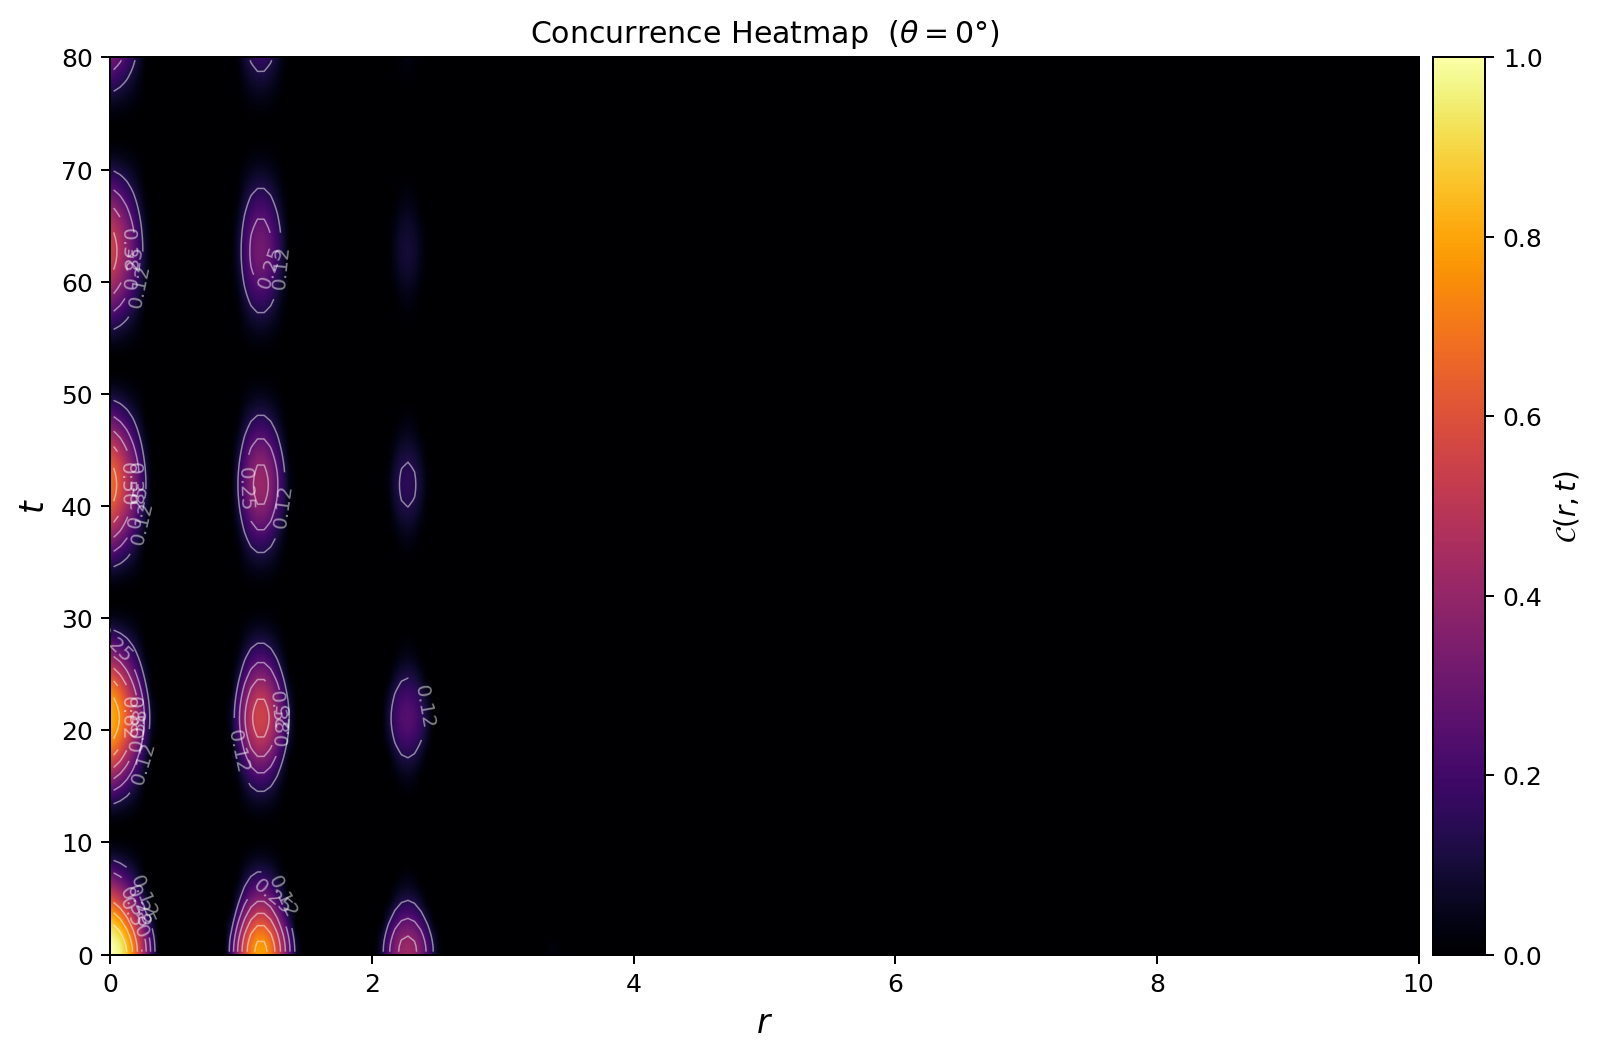
\includegraphics[width=0.92\textwidth]
    {figures/hubbard_amp_independent_gA4.50_GA0.010_gB4.50_GB0.010_C_heatmap.png}
    \caption{
    Concurrence $C(r,0^\circ,t)$ for independent non-Markovian amplitude
    damping with $\gamma_A=\gamma_B=4.5$ and $\Gamma_A=\Gamma_B=0.01$.
    The initial state uses $U/t=75$, $\Delta_t/t=4.5$, $V_{\mathrm{SO}}=0$,
    $n=1.875$, and $N_k=100$. The axes contain $200$ radial points on
    $0\leq r\leq10$ and $161$ time points on $0\leq t\leq80$. Dark regions
    denote $C=0$; the separated bright regions are nonzero-concurrence windows
    generated from the same spatial state and survival probability as the
    singlet fraction in Fig.~\ref{fig:F_high_heatmap}.
    }
    \label{fig:C_high_heatmap}
\end{figure*}

The singlet-referenced fidelity in Fig.~\ref{fig:F_high_heatmap} displays
related but nonidentical behavior. It remains nonzero in regions where the
concurrence has vanished, as expected because a mixed separable state can
retain singlet weight. At $r=0$, the initial state is a pure singlet and
independent amplitude damping gives the direct relations
\begin{equation}
F_{\mathrm s}(0,t)=p(t),
\qquad
C(0,t)=p(t).
\label{eq:r0_high}
\end{equation}
The two quantities therefore coincide at this special point. At finite
separation no such identity holds, and singlet weight can remain nonzero after
the X-state concurrence has vanished. The archived time slices give maxima
$F_{\mathrm s}=0.81091$, $0.65751$, and
$0.53309$ near $t=21$, $42$, and $63$, respectively, followed by a decreasing
envelope. At intervening survival-probability minima the singlet fraction
nearly vanishes.

\begin{figure*}[t]
    \centering
    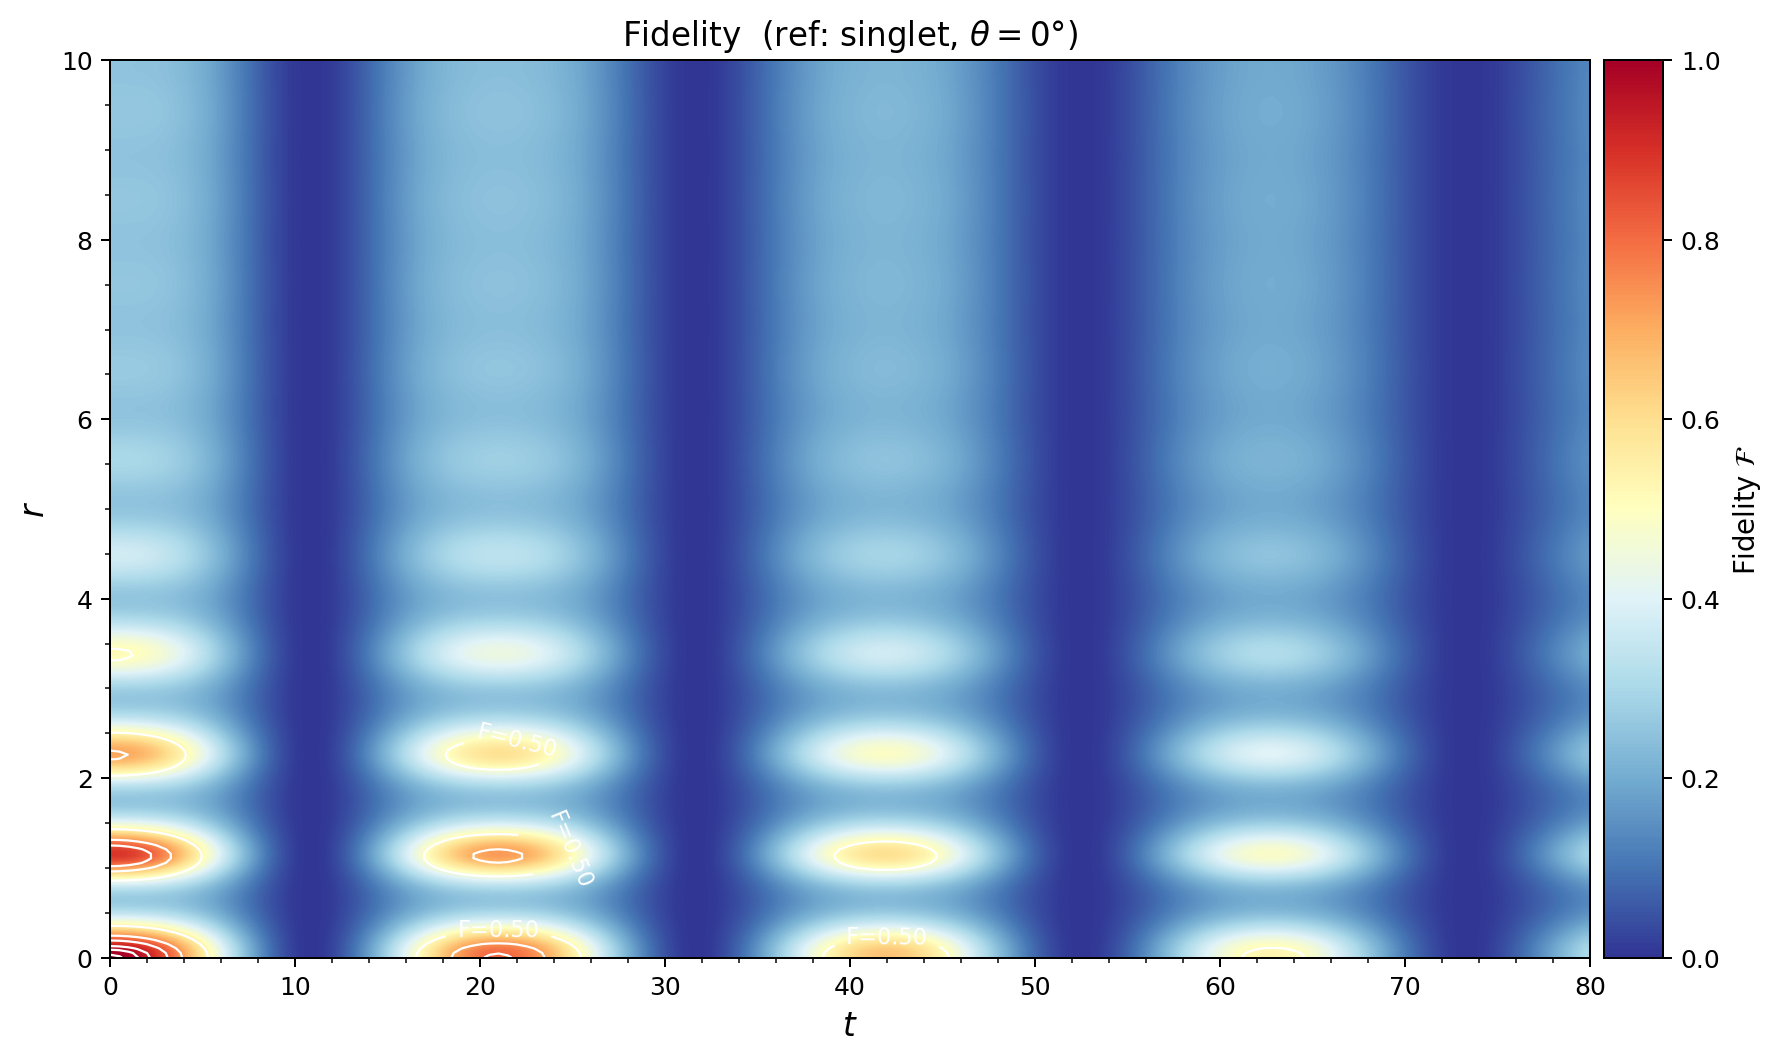
\includegraphics[width=0.92\textwidth]
    {figures/hubbard_amp_independent_gA4.50_GA0.010_gB4.50_GB0.010_F_heatmap_singlet.png}
    \caption{
    Singlet-referenced Uhlmann fidelity
    $\mathcal F_{\Psi^-}(r,0^\circ,t)=F_{\mathrm s}(r,0^\circ,t)$ for the same
    independent amplitude-damping regime and model settings as
    Fig.~\ref{fig:C_high_heatmap}. The color scale is the overlap with
    $|\Psi^-\rangle$, not fidelity to the initial mixed state and not an
    optimized average teleportation fidelity. The radial oscillations are
    inherited from the initial two-spin state, while the repeated temporal
    modulation follows $p(t)$. Contour lines are plotting guides and are not
    assigned operational teleportation thresholds.
    }
    \label{fig:F_high_heatmap}
\end{figure*}

The contrast between Figs.~\ref{fig:C_high_heatmap} and
\ref{fig:F_high_heatmap} illustrates why concurrence and singlet fraction
must be reported separately. Entanglement sudden death occurs whenever the
X-state concurrence condition fails, whereas $F_{\mathrm s}$ can remain
finite at finite separation. A nonmonotonic singlet fraction alone is therefore
insufficient to establish a revival of entanglement away from the special
zero-separation state.

\subsection{Fidelity dynamics at lower coupling}
\label{sec:fidelity_time}

Figure~\ref{fig:F_low_time} shows the singlet fraction for
$\gamma_A=\gamma_B=1.5$ and $\Gamma_A=\Gamma_B=0.1$ along $\theta=45^\circ$.
The selected separations are those generated by the plotting routine,
$r=0$, $1.9598$, $3.9698$, $5.9799$, $7.9899$, and $10$. All curves exhibit
damped nonmonotonic behavior associated with the same single-qubit survival
probability. At $r=0$, Eq.~\eqref{eq:r0_high} remains valid with the new
parameters; the first two sampled revival maxima are $0.31136$ at $t=11.6923$
and $0.09694$ at $t=23.3846$. Their decreasing magnitudes exclude any claim of
persistent or growing revivals over the computed interval.

\begin{figure}[t]
    \centering
    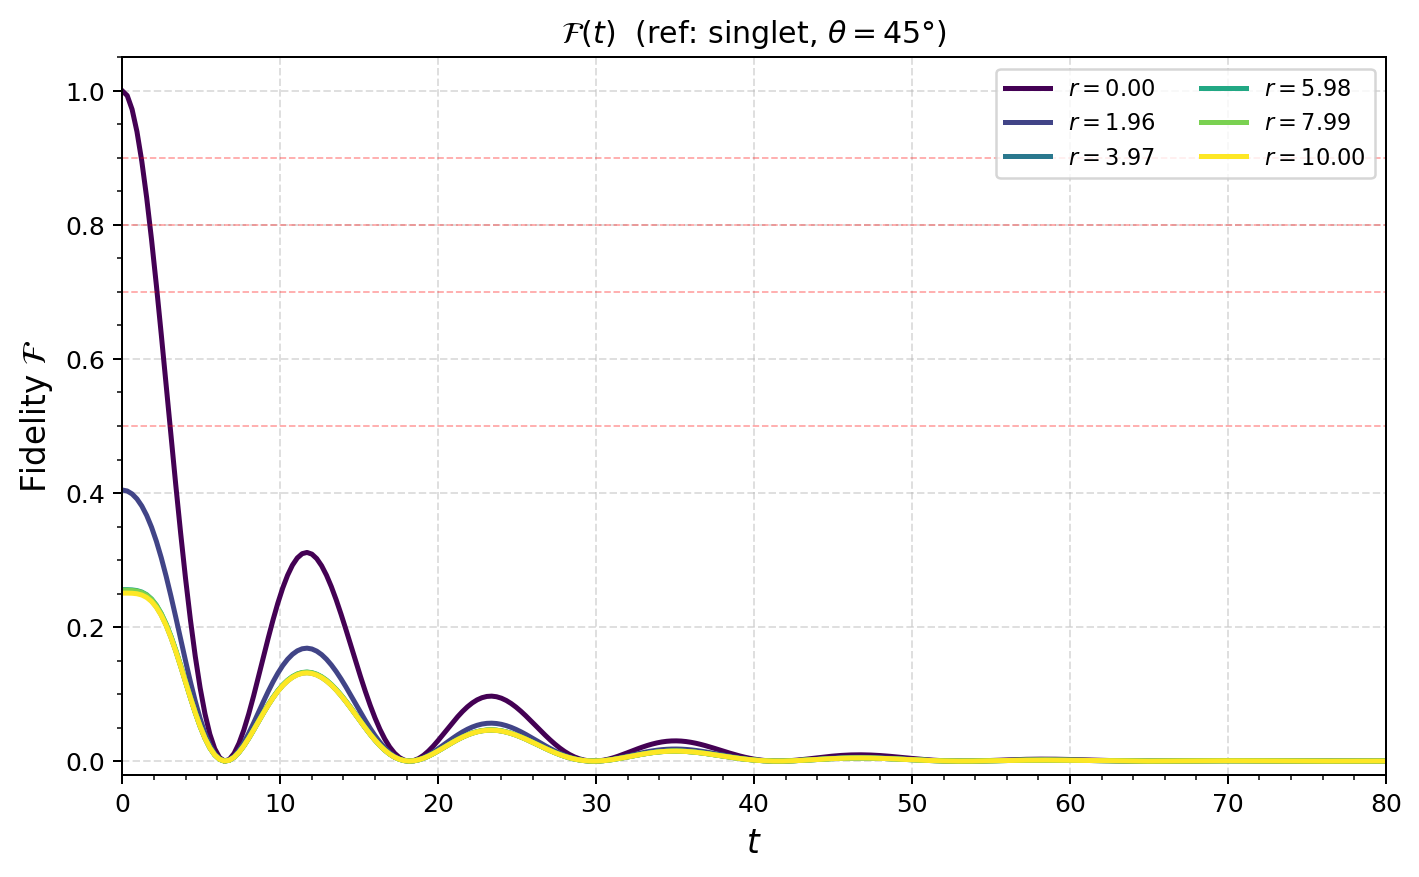
\includegraphics[width=\columnwidth]
    {figures/hubbard_amp_independent_gA1.50_GA0.100_gB1.50_GB0.100_F_vs_t_singlet.png}
    \caption{
    Time dependence of the singlet-referenced fidelity
    $\mathcal F_{\Psi^-}(r,45^\circ,t)=F_{\mathrm s}$ for independent
    amplitude damping with $\gamma_A=\gamma_B=1.5$ and
    $\Gamma_A=\Gamma_B=0.1$, using the common $U/t=75$ initial-state settings.
    The data contain $261$ times on $0\leq t\leq80$. The horizontal dashed
    lines at $0.5$, $0.7$, $0.8$, and $0.9$ are automatically drawn reference
    guides; they are not thresholds for the plotted singlet fraction.
    }
    \label{fig:F_low_time}
\end{figure}

The large-$r$ curves begin close to one quarter, consistent with a Werner
state whose singlet weight approaches the maximally mixed value
$F_{\mathrm s}=1/4$ as $p\to0$. Their subsequent time dependence is dominated
by the common noise channel rather than by a persistent long-range entangled
resource. At all displayed separations, the singlet fraction approaches zero
at long times because the amplitude-damping fixed point is a ground-state
product state orthogonal to $|\Psi^-\rangle$. This fixed-point statement does
not apply to fidelity to each initial state, which is a different array in the
repository.

\subsection{Angular dependence of the singlet fraction}
\label{sec:fidelity_angular}

Angular dependence enters the calculation only through
$\mathbf r=r(\cos\theta,\sin\theta)$ in the Green's functions and hence through
$\rho(\mathbf r,0)$. The amplitude-damping Kraus operators and $p(t)$ contain no
angle-dependent coefficient. Consequently, the noise does not introduce a new
preferred lattice direction; angular structure at finite time is inherited
from the initial state and modified by the common temporal map.

Figure~\ref{fig:F_angular} displays the initial singlet fraction at seven
sampled angles and four separations. The $r=0$ curve is unity at every angle,
as required by $p(\mathbf0)=1$. Nontrivial anisotropy is visible at finite
separation. For example, at $r=3.3166$ the initial singlet fraction ranges
from $0.25190$ at $30^\circ$ and $60^\circ$ to $0.50801$ at $45^\circ$. At
$r=6.6332$ and $10$, the corresponding angular ranges are much smaller,
approximately $0.01616$ and $0.00154$, respectively. The sampled data obey
$F_{\mathrm s}(0^\circ)=F_{\mathrm s}(90^\circ)$,
$F_{\mathrm s}(15^\circ)=F_{\mathrm s}(75^\circ)$, and
$F_{\mathrm s}(30^\circ)=F_{\mathrm s}(60^\circ)$ to numerical precision.

\begin{figure}[t]
    \centering
    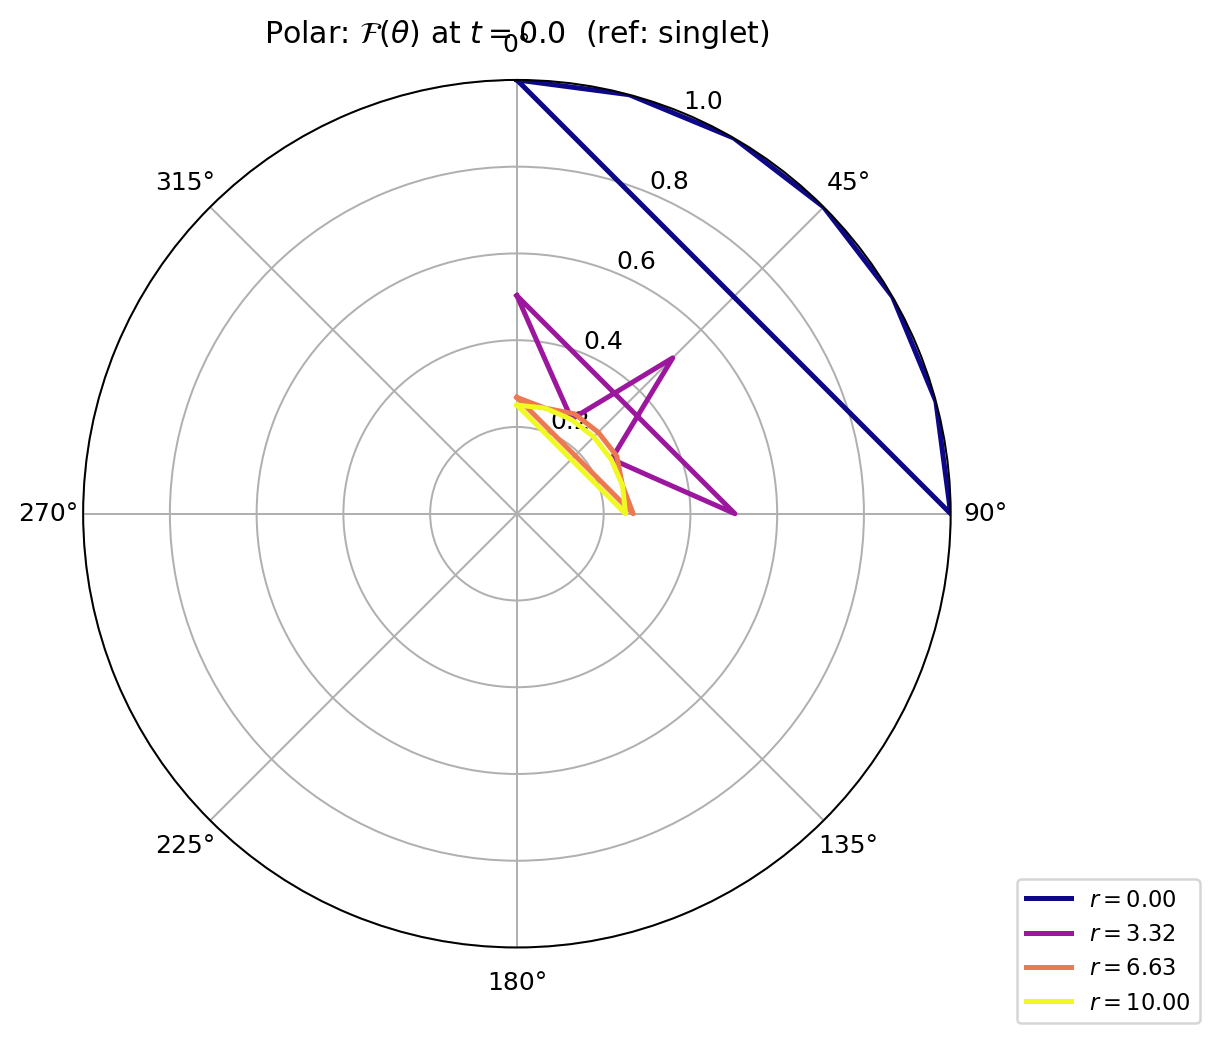
\includegraphics[width=\columnwidth]
    {figures/hubbard_amp_independent_gA1.50_GA0.100_gB1.50_GB0.100_F_polar_singlet.png}
    \caption{
    Polar representation of the initial singlet fraction
    $F_{\mathrm s}(r,\theta,0)$ for $r=0$, $3.3166$, $6.6332$, and $10$ in the
    $\gamma=1.5$, $\Gamma=0.1$ data set. Only
    $\theta=0^\circ,15^\circ,\ldots,90^\circ$ were simulated. The plotted
    closure between $90^\circ$ and $0^\circ$ is a line connecting the sampled
    endpoints, and the unpopulated remainder of the polar circle must not be
    interpreted as additional angular data. The radial coordinate is the
    singlet fraction, not the electron separation.
    }
    \label{fig:F_angular}
\end{figure}

These observations support an initial-state lattice anisotropy at selected
finite separations, not a universal preferred direction at all $r$. Nor does
the angle-independent $r=0$ curve establish isotropy of the finite-$r$ state.
Because only the first quadrant was sampled, no independent conclusion about
unsampled angles is drawn beyond the lattice symmetries explicitly tested by
the available grid.

\subsection{Holevo information and dense coding}
\label{sec:holevo_results}

The spatial behavior of the Pauli-ensemble Holevo quantity is shown in
Fig.~\ref{fig:holevo_spatial} for $\theta=45^\circ$. At $t=0$,
$\chi_{\mathrm P}=2$ bits at $r=0$, as required for a pure singlet. The initial
curve then falls below one bit before displaying a finite-separation maximum
of $1.06735$ bits at $r=1.6080$. Subsequent sampled maxima at $r=3.2161$ and
$4.8241$ are $0.27961$ and $0.03566$ bits, respectively. Thus the initial
spatial profile is nonmonotonic, but only the zero-separation region and the
first finite-$r$ maximum exceed the one-bit benchmark in this angular slice.

\begin{figure}[t]
    \centering
    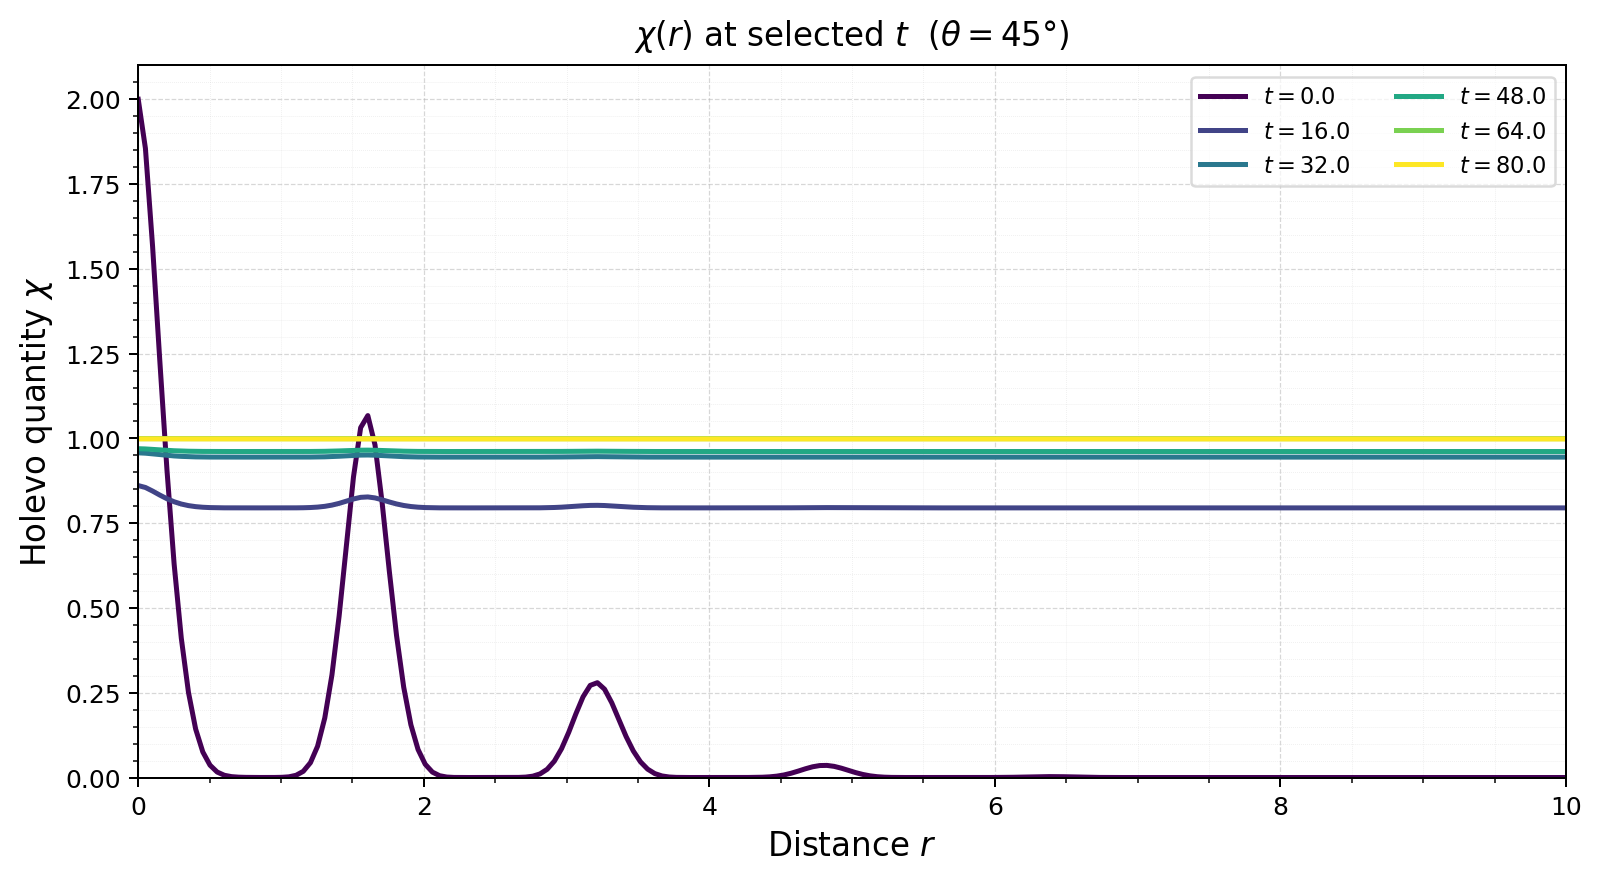
\includegraphics[width=\columnwidth]
    {figures/hubbard_amp_independent_gA1.50_GA0.100_gB1.50_GB0.100_holevo_vs_r.png}
    \caption{
    Pauli-ensemble Holevo quantity $\chi_{\mathrm P}(r,45^\circ,t)$ at
    $t=0,16,32,48,64,80$ for independent amplitude damping with
    $\gamma_A=\gamma_B=1.5$, $\Gamma_A=\Gamma_B=0.1$, and the common $U/t=75$
    initial-state settings. Entropies use base-two logarithms. The quantity is
    defined by Eqs.~\eqref{eq:holevo_definition} and
    \eqref{eq:holevo_entropy}; it is not concurrence or singlet fidelity.
    }
    \label{fig:holevo_spatial}
\end{figure}

The temporal slices flatten toward one bit, with small finite-time deviations
still visible in the arrays. This tendency follows from the amplitude-damping
fixed point derived below Eq.~\eqref{eq:holevo_entropy}, rather than from a
survival of dense-coding quantum advantage. Indeed, the asymptotic value one
is precisely the classical one-qubit benchmark. At $t=16$, for example, the
sampled radial range is $0.79509$--$0.86087$ bits, below that benchmark
throughout this slice.

Figure~\ref{fig:holevo_angular} resolves the angular and temporal behavior at
$r=0$. The initial value is two bits at every sampled angle. Subsequent
oscillations are identical across the seven angular rows to numerical
precision. This angle independence is expected because the zero-separation
initial state is the same pure singlet for every row and the independent noise
channel is angle independent. The figure therefore verifies the consistency
of the $r=0$ slice; it does not demonstrate that $\chi_{\mathrm P}$ is angle
independent at finite $r$, where the initial state is anisotropic.

\begin{figure*}[t]
    \centering
    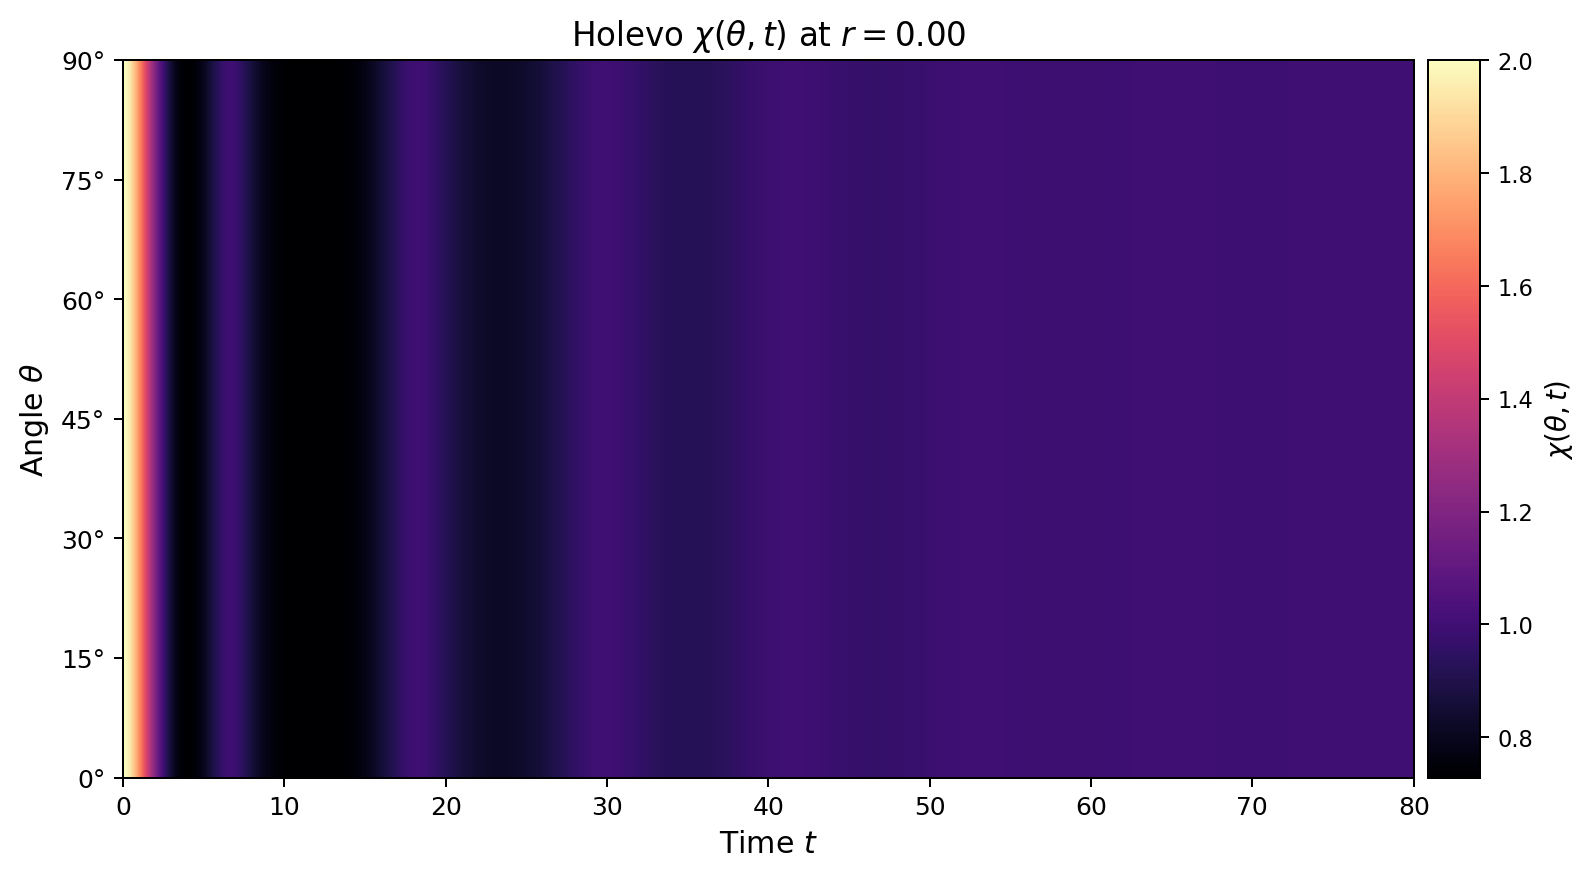
\includegraphics[width=0.92\textwidth]
    {figures/hubbard_amp_independent_gA1.50_GA0.100_gB1.50_GB0.100_holevo_theta_t_heatmap.png}
    \caption{
    Pauli-ensemble Holevo quantity $\chi_{\mathrm P}(\theta,r=0,t)$ for the
    same $\gamma=1.5$, $\Gamma=0.1$ regime as
    Fig.~\ref{fig:holevo_spatial}. The seven rows correspond to
    $\theta=0^\circ,15^\circ,\ldots,90^\circ$, and $261$ time points span
    $0\leq t\leq80$. The identical rows follow from the angle-independent
    pure-singlet initial state at $r=0$ and the angle-independent local Kraus
    map; no finite-separation isotropy is implied.
    }
    \label{fig:holevo_angular}
\end{figure*}

The Holevo dynamics differ markedly from the singlet-fidelity dynamics in
Fig.~\ref{fig:F_low_time}. Whereas the singlet fraction tends to zero with the
ground-state product fixed point, $\chi_{\mathrm P}$ tends to one bit. During
intermediate times it can fall below one and subsequently return toward one as
the state becomes less mixed. Such an increase toward the classical benchmark
must not be described as a revival of entanglement or as an increase above the
dense-coding classical limit. More generally, Eq.~\eqref{eq:holevo_entropy}
shows that the dynamics are controlled by both the global entropy and the
subsystem entropy, so identical behavior of concurrence, singlet fraction, and
Holevo information is not expected.

\subsection{Hubbard interaction dependence of fidelity and Holevo information}
\label{sec:U_results}

The Hubbard interaction enters Eq.~\eqref{eq:interaction}, changes the
self-consistent triple $(\Delta_0,\Delta_s,\mu)$, and thereby modifies
$E_{\mathbf ks}$, the Green's functions, and the initial Werner parameter.
The open-system Kraus operators themselves contain no $U$. Consequently, any
computed dependence
$\mathcal F(U,\theta,r,t)$ or $\chi_{\mathrm P}(U,\theta,r,t)$ is transmitted
through the initial state and then acted upon by a $U$-independent noise map.

To test this dependence numerically, we performed a new sweep at the three
interaction strengths already used in Fig.~\ref{fig:delta_ks_heatmaps}:
$U/t=40$, $75$, and $115$. All other model parameters were fixed, and each
self-consistency solution satisfied the residual criterion reported in
Sec.~\ref{sec:validation}. For each interaction strength we used the full
seven-angle, $200$-radius, and $261$-time grid in the
$\gamma_A=\gamma_B=1.5$, $\Gamma_A=\Gamma_B=0.1$ independent-amplitude-damping
regime. Concurrence, singlet fraction, and the Pauli-ensemble Holevo quantity
were evaluated with the same validated formulas. The initial density matrices
were Hermitian, normalized, and positive semidefinite. The complete arrays,
self-consistency parameters, residuals, and commit identifier are stored in
the accompanying NPZ file.

\begin{figure*}[t]
    \centering
    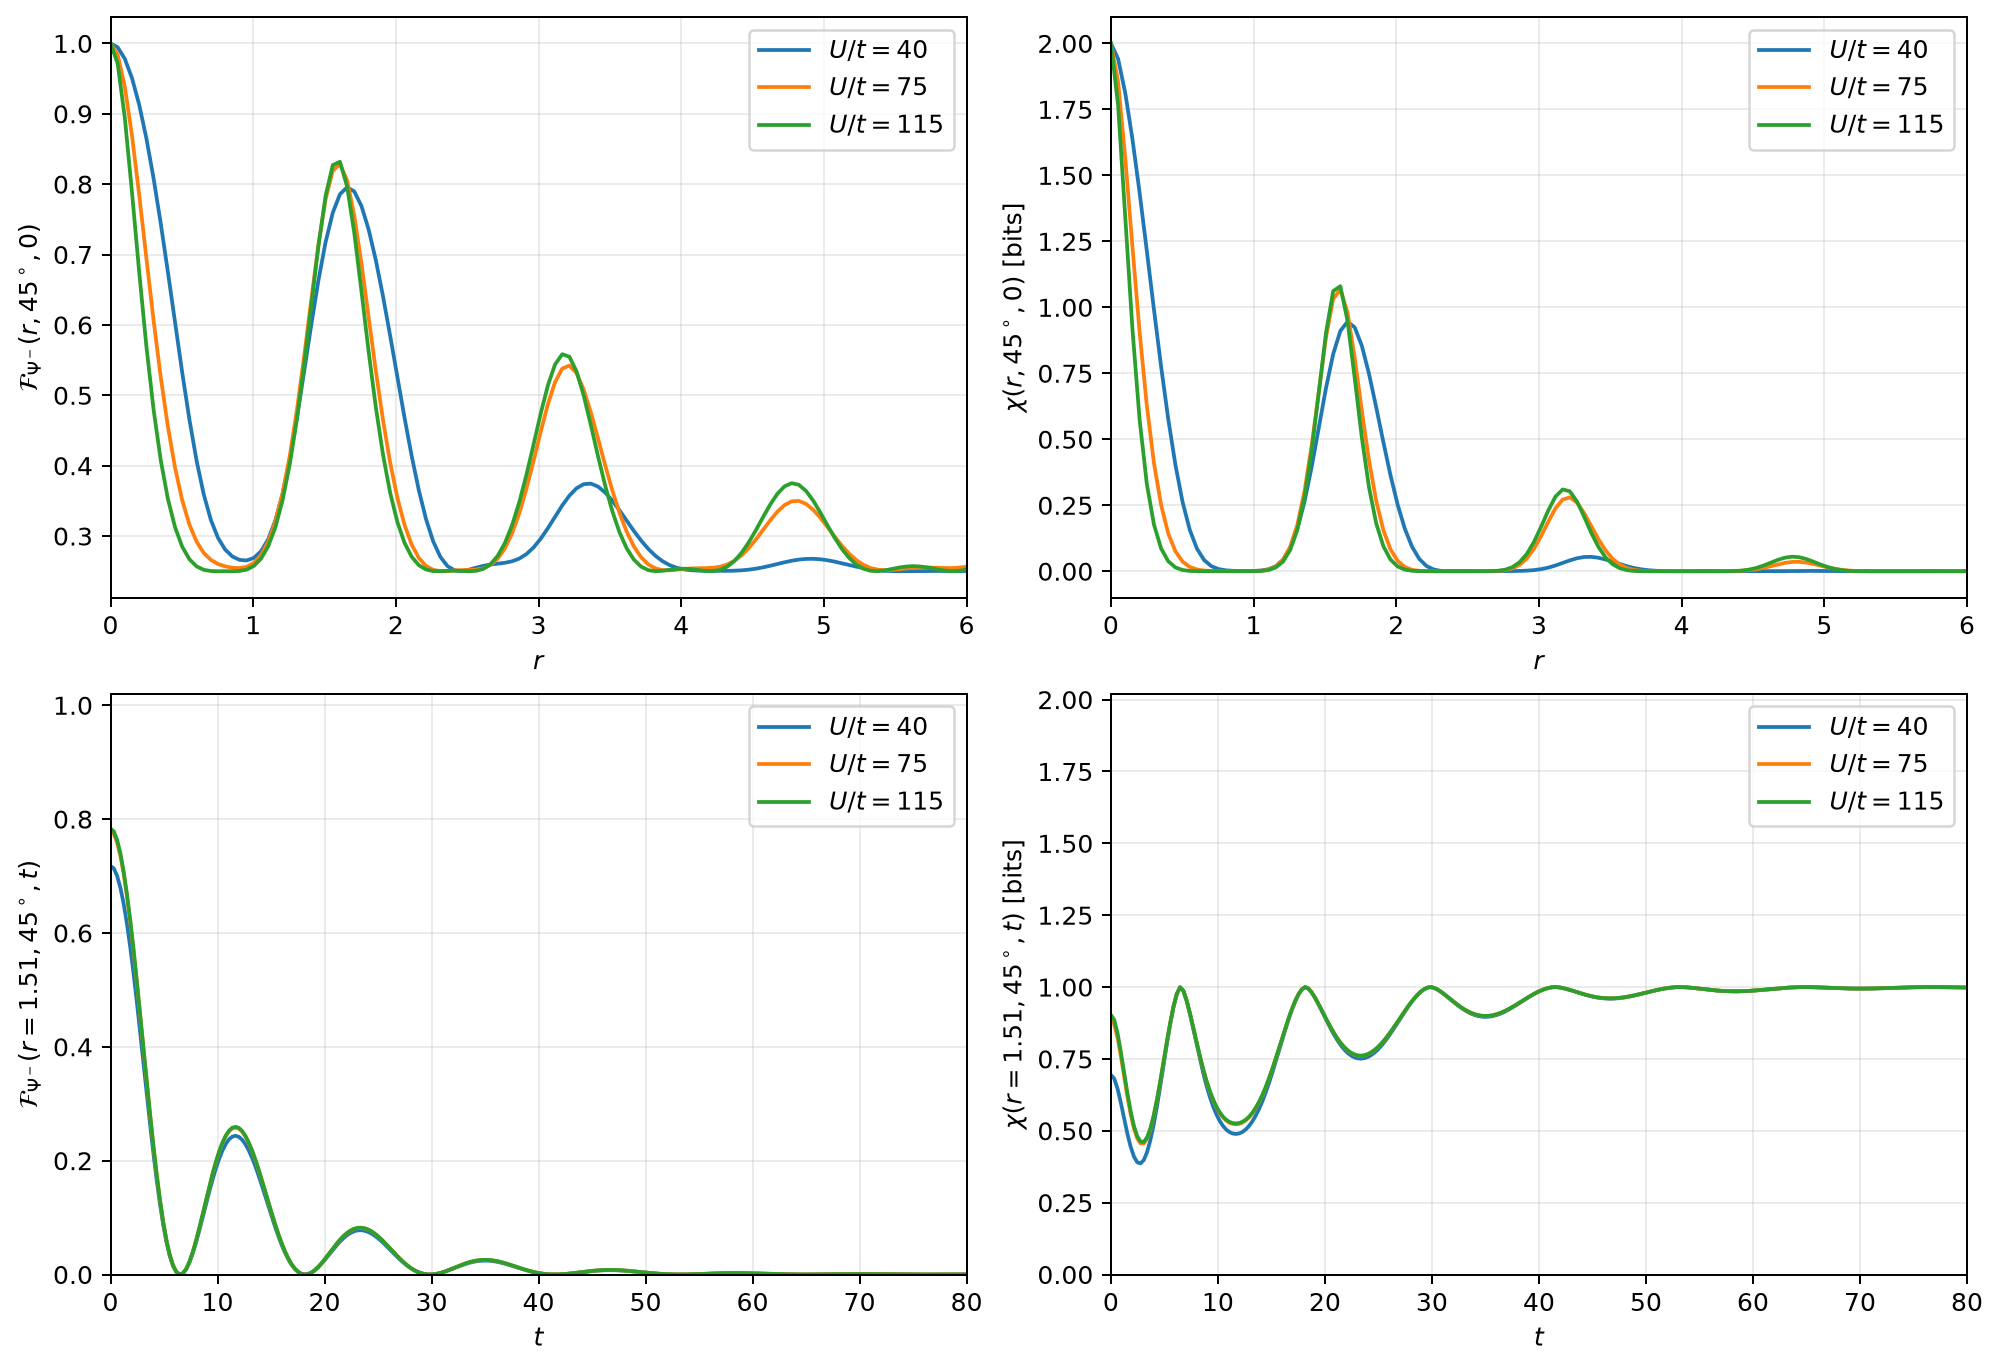
\includegraphics[width=0.94\textwidth]
    {figs/U_dependence_fidelity_holevo.png}
    \caption{
    Interaction dependence computed for $U/t=40$, $75$, and $115$ in the
    $\gamma_A=\gamma_B=1.5$, $\Gamma_A=\Gamma_B=0.1$ regime. Upper panels:
    initial singlet fraction and Pauli-ensemble Holevo quantity along
    $\theta=45^\circ$. Lower panels: their time dependence at the fixed sampled
    separation $r=1.50754$ and the same angle. All other BdG parameters are
    identical to those in Fig.~\ref{fig:delta_ks_heatmaps}. The interaction
    changes the initial state but does not enter the Kraus map. These results
    use the repository's magnitude-amplitude Green's-function convention.
    }
    \label{fig:U_fidelity_holevo}
\end{figure*}

The upper panels of Fig.~\ref{fig:U_fidelity_holevo} show that $U$ modifies
both the positions and amplitudes of the spatial structures. The ordering is
separation dependent. At $r=0.50251$, for example, the initial singlet
fraction decreases from $0.53243$ at $U/t=40$ to $0.350996$ at $75$ and
$0.284845$ at $115$; the corresponding Holevo values are $0.26196$,
$0.03640$, and $0.00454$ bits. At $r=1.50754$, by contrast, the singlet
fraction increases across the same three interactions, taking values
$0.717745$, $0.778551$, and $0.783515$, while $\chi_{\mathrm P}$ takes values
$0.694131$, $0.886208$, and $0.903183$ bits. These paired examples directly
rule out a universal monotonic enhancement or suppression over the spatial
domain.

The lower panels show the consequences at fixed $r=1.50754$. The singlet
fraction exhibits damped revivals at common times because $p(t)$ is shared;
the interaction changes the initial amplitude and therefore the detailed
curve, but does not introduce a separate environmental timescale. The Holevo
curves likewise approach one bit at long times, with nearly indistinguishable
late-time behavior on the plotted scale. At $r=0$, all three interactions
instead give exactly the same curves because the zero-separation initial
state is the pure singlet for every converged solution.

The supported conclusion is therefore specific: within the three-point,
fixed-filling, magnitude-amplitude calculation, the Hubbard interaction
changes the initial spatial correlations and thereby changes the subsequent
singlet-fidelity and Pauli-Holevo dynamics. The data do not establish a global
functional law in $U$, an optimal interaction strength, or a universally
beneficial interaction effect. A denser sweep and a comparative implementation
of the signed coherence factor would be required before extending these
conclusions beyond the present implementation and parameter set.

\section{Conclusion}

We have examined the Green's-function construction of two-spin BCS density
matrices and their subsequent independent non-Markovian amplitude-damping
dynamics. The exact signed BdG identity
$u_{\mathbf ks}v_{\mathbf ks}^*=-\Delta_{\mathbf ks}^*/2E_{\mathbf ks}$ must
be distinguished from the repository's legacy unsigned-amplitude numerical
implementation. We have also shown that taking the absolute value of an
already real normalized Green's-function ratio does not itself alter the
present density matrix, which depends only on $g^2$ and $f^2$; the physically
important difference is whether the gap sign is retained before momentum
integration.

The archived results establish spatially structured concurrence and singlet
fraction, with temporal revivals determined by the oscillatory survival
probability in the two underdamped regimes considered. Singlet-referenced
Uhlmann fidelity is exactly the singlet fraction, but it is not an optimized
teleportation fidelity for the evolved states. The equal-probability Pauli
encoding satisfies $\bar\rho_{AB}=(I_A/2)\otimes\rho_B$ and hence
$\chi_{\mathrm P}=1+S_2(\rho_B)-S_2(\rho_{AB})$. Its approach to one bit at
long times reflects the pure product fixed point and does not represent a
residual dense-coding quantum advantage. Angular structure is inherited from
the initial Green's functions, not introduced by the angle-independent noise.

The converged sweep at $U/t=40$, $75$, and $115$ demonstrates
interaction-dependent modifications of the initial and evolved information
measures within the implemented convention. Their ordering changes with
separation, precluding a universal claim of interaction-induced enhancement or
suppression.

The independent corrected equal-time density study further shows that lowering
$U$ can create large nonzero-gap stationary branches at low density: all seven
fillings are paired at $U/t=15$, whereas $U/t=25$ is paired for $n\geq1$ on the
production mesh. This does not translate into useful finite-site
teleportation. All 140 tested nonzero production states have zero concurrence,
and the largest exact-site average fidelity is $0.636508$, below $2/3$.
Normal exchange can define a conditional Werner resource without
superconductivity, while a large anomalous correlator does not guarantee an
operational advantage. Continuous critical radii below $a$ have not been
interpreted as physical sub-lattice separations, and stationary BdG branches
have not been identified with global free-energy minima.

The principal remaining tasks are a unified signed-Green's-function
regeneration of the legacy open-system dynamics, a parameter-preserving
evolution pipeline for all observables, locally optimized fully entangled
fractions for general evolved states, and free-energy or competing-order
analyses before assigning thermodynamic phase stability.

\begin{acknowledgments}
Numerical results were obtained with a self-consistent BdG solver and open-quantum-system evolution code implemented by the author.
\end{acknowledgments}

\begin{thebibliography}{99}

\bibitem{Oh2004}
S. Oh and J. Kim, Entanglement of electron spins of non-interacting electron gases, Phys.\ Rev.\ A \textbf{69}, 054305 (2004).

\bibitem{Oh2005}
S. Oh and J. Kim, Entanglement of electron spins in superconductors, Phys.\ Rev.\ B \textbf{71}, 144523 (2005).

\bibitem{Bennett1993}
C. H. Bennett, G. Brassard, C. Cr\'epeau, R. Jozsa, A. Peres, and W. K. Wootters, Teleporting an unknown quantum state via dual classical and Einstein-Podolsky-Rosen channels, Phys.\ Rev.\ Lett.\ \textbf{70}, 1895 (1993).

\bibitem{BennettWiesner1992}
C. H. Bennett and S. J. Wiesner, Communication via one- and two-particle operators on Einstein-Podolsky-Rosen states, Phys.\ Rev.\ Lett.\ \textbf{69}, 2881 (1992).

\bibitem{Wootters1998}
W. K. Wootters, Entanglement of formation of an arbitrary state of two qubits, Phys.\ Rev.\ Lett.\ \textbf{80}, 2245 (1998).

\bibitem{Jozsa1994}
R. Jozsa, Fidelity for mixed quantum states, J.\ Mod.\ Opt.\ \textbf{41}, 2315 (1994).

\bibitem{Horodecki1999}
M. Horodecki, P. Horodecki, and R. Horodecki, General teleportation channel, singlet fraction, and quasidistillation, Phys.\ Rev.\ A \textbf{60}, 1888 (1999).

\bibitem{Bruss2004}
D. Bru\ss, G. M. D'Ariano, M. Lewenstein, C. Macchiavello, A. Sen(De), and U. Sen, Distributed quantum dense coding, Phys.\ Rev.\ Lett.\ \textbf{93}, 210501 (2004).

\bibitem{Breuer2002}
H.-P. Breuer and F. Petruccione, \emph{The Theory of Open Quantum Systems} (Oxford University Press, Oxford, 2002).

\bibitem{Bellomo2007}
B. Bellomo, R. Lo Franco, and G. Compagno, Non-Markovian effects on the dynamics of entanglement, Phys.\ Rev.\ Lett.\ \textbf{99}, 160502 (2007).

\end{thebibliography}

\end{document}
